\chapter{Dark matter overview}\label{chap:DarkMatterOverview}
One of the most compelling mysteries in physics and cosmology is the nature of dark matter. Observational evidence strongly suggests the presence of a non-luminous, non-baryonic form of matter that constitutes the majority of the mass in the Universe. Dark matter has so far eluded experimental searches, and its underlying composition remains unknown. This chapter provides an overview of the observational evidence supporting its existence in \autoref{sec:DMOverview/Evidence4DM}. This is followed by a discussion of an alternative to dark matter based on a modification of Newtonian dynamics in \autoref{sec:DMOverview/MOND}. Various particle candidates proposed to explain the existence of non-baryonic dark matter are discussed in \autoref{sec:DMOverview/Candidates4DM}, followed in \autoref{sec:DMOverview/DetectionOfDM} by the possible detection mechanisms and the experiments currently searching for dark matter.

\section{Evidence for dark matter}\label{sec:DMOverview/Evidence4DM}
In the latter part of the 19th century, astronomers began to propose the existence of non-luminous matter to account for the uneven distribution of stars observed in the night sky \cite{HistoryofDM}. One of the earliest quantitative attempts to estimate the presence of such "dark bodies" in the Milky Way was made by Lord Kelvin in 1904. Kelvin postulated that if stars in the Milky Way could be modelled analogously to particles in a gas, interacting primarily through gravity, then a relationship could be established between the size of the system and the velocity dispersion of its constituents \cite{Kelvin1904}. The term \textit{dark matter} (\textit{mati\`ere obscure}) was first introduced by Henri Poincar\`e in 1906. Based on Kelvin’s velocity dispersion calculations, Poincar\`e argued that the amount of dark matter was likely to be less than or equal to the amount of visible matter \cite{HPon}. In 1922, Jacobus Kapteyn developed one of the earliest models to quantitatively describe the size and structure of the Milky Way. His model characterized the stellar distribution as a flattened disk rotating about an axis aligned with the galactic pole. Kapteyn reached conclusions similar to those of Poincaré, asserting that the presence of significant quantities of unseen matter was improbable \cite{Kapteyn1922}.

While these early investigations did not yield definitive evidence for the existence of dark matter, they established a foundational framework upon which later studies would build more rigorous arguments for the presence of missing mass in the Galaxy.

\subsection{Virial theorem and the Coma Cluster}\label{sec:DMOverview/ViralTheorem}
The virial theorem is a fundamental result in classical mechanics that relates the average total kinetic energy $\langle T \rangle$ of a system to its average total potential energy $\langle U \rangle$. The theorem can be used to estimate the mass of a galaxy cluster through the following approximation:
\begin{equation}
\begin{split}
2\langle T \rangle + \langle U \rangle = 0, \\
Nm\langle v^2\rangle - \frac{3}{5}\frac{GN^2m^2}{R}=0,\\
Nm=\frac{5R\langle v_r^2 \rangle}{G}\\
\end{split}
\label{eq:DMOverview/virial}
\end{equation}
where $N$ is the estimated number of galaxies in the cluster, each having an observed stellar mass $m$, $v_r$ is the radial velocities, and $R$ is the radius of the cluster.

In 1933, Fritz Zwicky applied the virial theorem to the Coma Cluster of galaxies \cite{Zwicky1933}. He measured the radial velocities of galaxies within the cluster and estimated their velocity dispersion. When he used the virial theorem to estimate the total mass required to gravitationally bind the system, he estimated the minimum mass of the galaxies in the cluster to be $m=4\times 10^{10}M_{\odot}$, where $M_{\odot}$ is one solar mass. With an average velocity dispersion observed to be approximately 1000~kms$^{-1}$, the mass-to-light ratio that was far too large to be accounted for by visible matter alone \cite{HistoryofDM}. Zwicky’s analysis revealed that the total mass inferred from the virial theorem was roughly 400 times greater than what could be explained by the luminous matter. To resolve this discrepancy, he proposed the existence of a substantial amount of unseen mass, which he referred to as \textit{dunkle Materie}, or “dark matter” \cite{Zwicky1933}.

\subsection{Galaxy rotation curves}\label{sec:DMOverview/RotationCurves}
A galaxy rotation curve describes the variation of orbital velocity of stars and gas as a function of their radial distance from the galactic centre. Under the assumption that a galaxy's mass is distributed entirely within its luminous matter, one would expect the mass to be concentrated primarily near the galactic centre. Therefore, the orbital velocity of objects situated at large radii should decrease with distance, according a Keplerian dynamics given by:
\begin{equation}
v(r) \propto \frac{1}{\sqrt{r}},
\end{equation}
where $v(r)$ is the orbital velocity and $r$ is the radial distance from the galactic centre.
In 1978, Vera C. Rubin \textit{et al.}\cite{Rubin} analysed the hydrogen spectra from a sample of ten high-luminosity spiral galaxies. By measuring the Doppler shift of the 21~cm line in the hydrogen spectra, they were able to determine the rotation velocities of gas and stars across a range of galactic radii. Rubin found that the rotation curves of these galaxies remained approximately constant, whilst the orbital velocities stayed constant, even at large radii. This observation was inconsistent with the mass inferred from visible matter alone and the expectations resulting from applied Keplerian dynamics.
A representative velocity profile for the galaxy NGC 6503 is shown in \autoref{fig:DMOverview/NGC6503}. The high orbital velocities at large radii suggests that a significant portion of galactic mass must be distributed well beyond the visible edge. This led to the hypothesis of a surrounding, non-luminous mass component, commonly referred to as a dark matter ``halo'' that provides the additional gravitational influence required to maintain the observed rotation velocities. The presence of such halo could explain the observed phenomena.
\begin{figure}[ht]
	\centering
	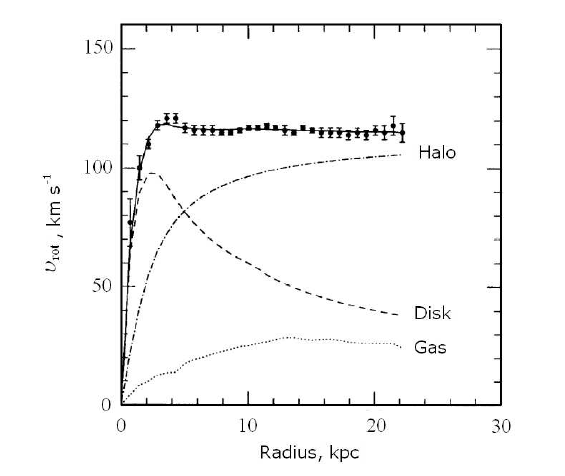
\includegraphics[width = 0.6\textwidth]{figures/DMOverview/NGC_6503.png}
	\caption[Galactic rotation curve for NGC 6503.]{Galactic rotation curve for NGC 6503. The dotted and dashed lines represents where the data should lie if Keplerian dynamics are obeyed. The dot-dashed line indicates the dark matter `halo' contribution needed for the function to fit the data. Figured reprinted from Ref.~\cite{Freese2009}.}
	\label{fig:DMOverview/NGC6503}
\end{figure}
\subsection{Gravitational lensing}\label{sec:DMOverview/GravLens}
The observed effect of gravitational lensing can be used to infer the total mass of astronomical objects. An example of the effect gravitational lensing has on light from a distant galaxy is shown in \autoref{fig:DMOverview/GravLens}. The effect was first described theoretically by Albert Einstein in 1936 \cite{GravLens}. The effect occurs when a massive object (lensing object) is situated in the line of sight between a distant source and an observer. Due to the gravitational field of the lensing object, light from the source deflects from its path resulting in observable distortions such as magnification, image splitting, or the formation of arcs and rings.
When the lensing is strong enough to produce multiple images or highly distorted arcs, it is referred to as \textit{strong gravitational lensing}. An example of such an effect is shown in \autoref{fig:DMOverview/StrongGravLens}. 

The degree of light deflection depends on the gravitational potential of the lensing object, which can be reconstructed by analysing the extent and geometry of the observed distortions \cite{Young2016}. 

The mass of the lensing object in the line of sight is compared with that of the observed baryonic matter (stars, dust and gas), and the existence of dark matter is inferred to explain the discrepancy between the visible mass and lensing mass. 

Notable examples of clusters which exhibit such properties are the Coma Cluster \cite{Briel:1997hz}, Abell 370 \cite{Natarajan:2024iqm}, MACS J1206 \cite{GravLensPicture} shown in \autoref{fig:DMOverview/GravLens} and the Bullet Cluster \cite{Clowe2006} shown in \autoref{fig:DMOverview/BulletCluster}.
\begin{figure}[ht!]
	\centering
	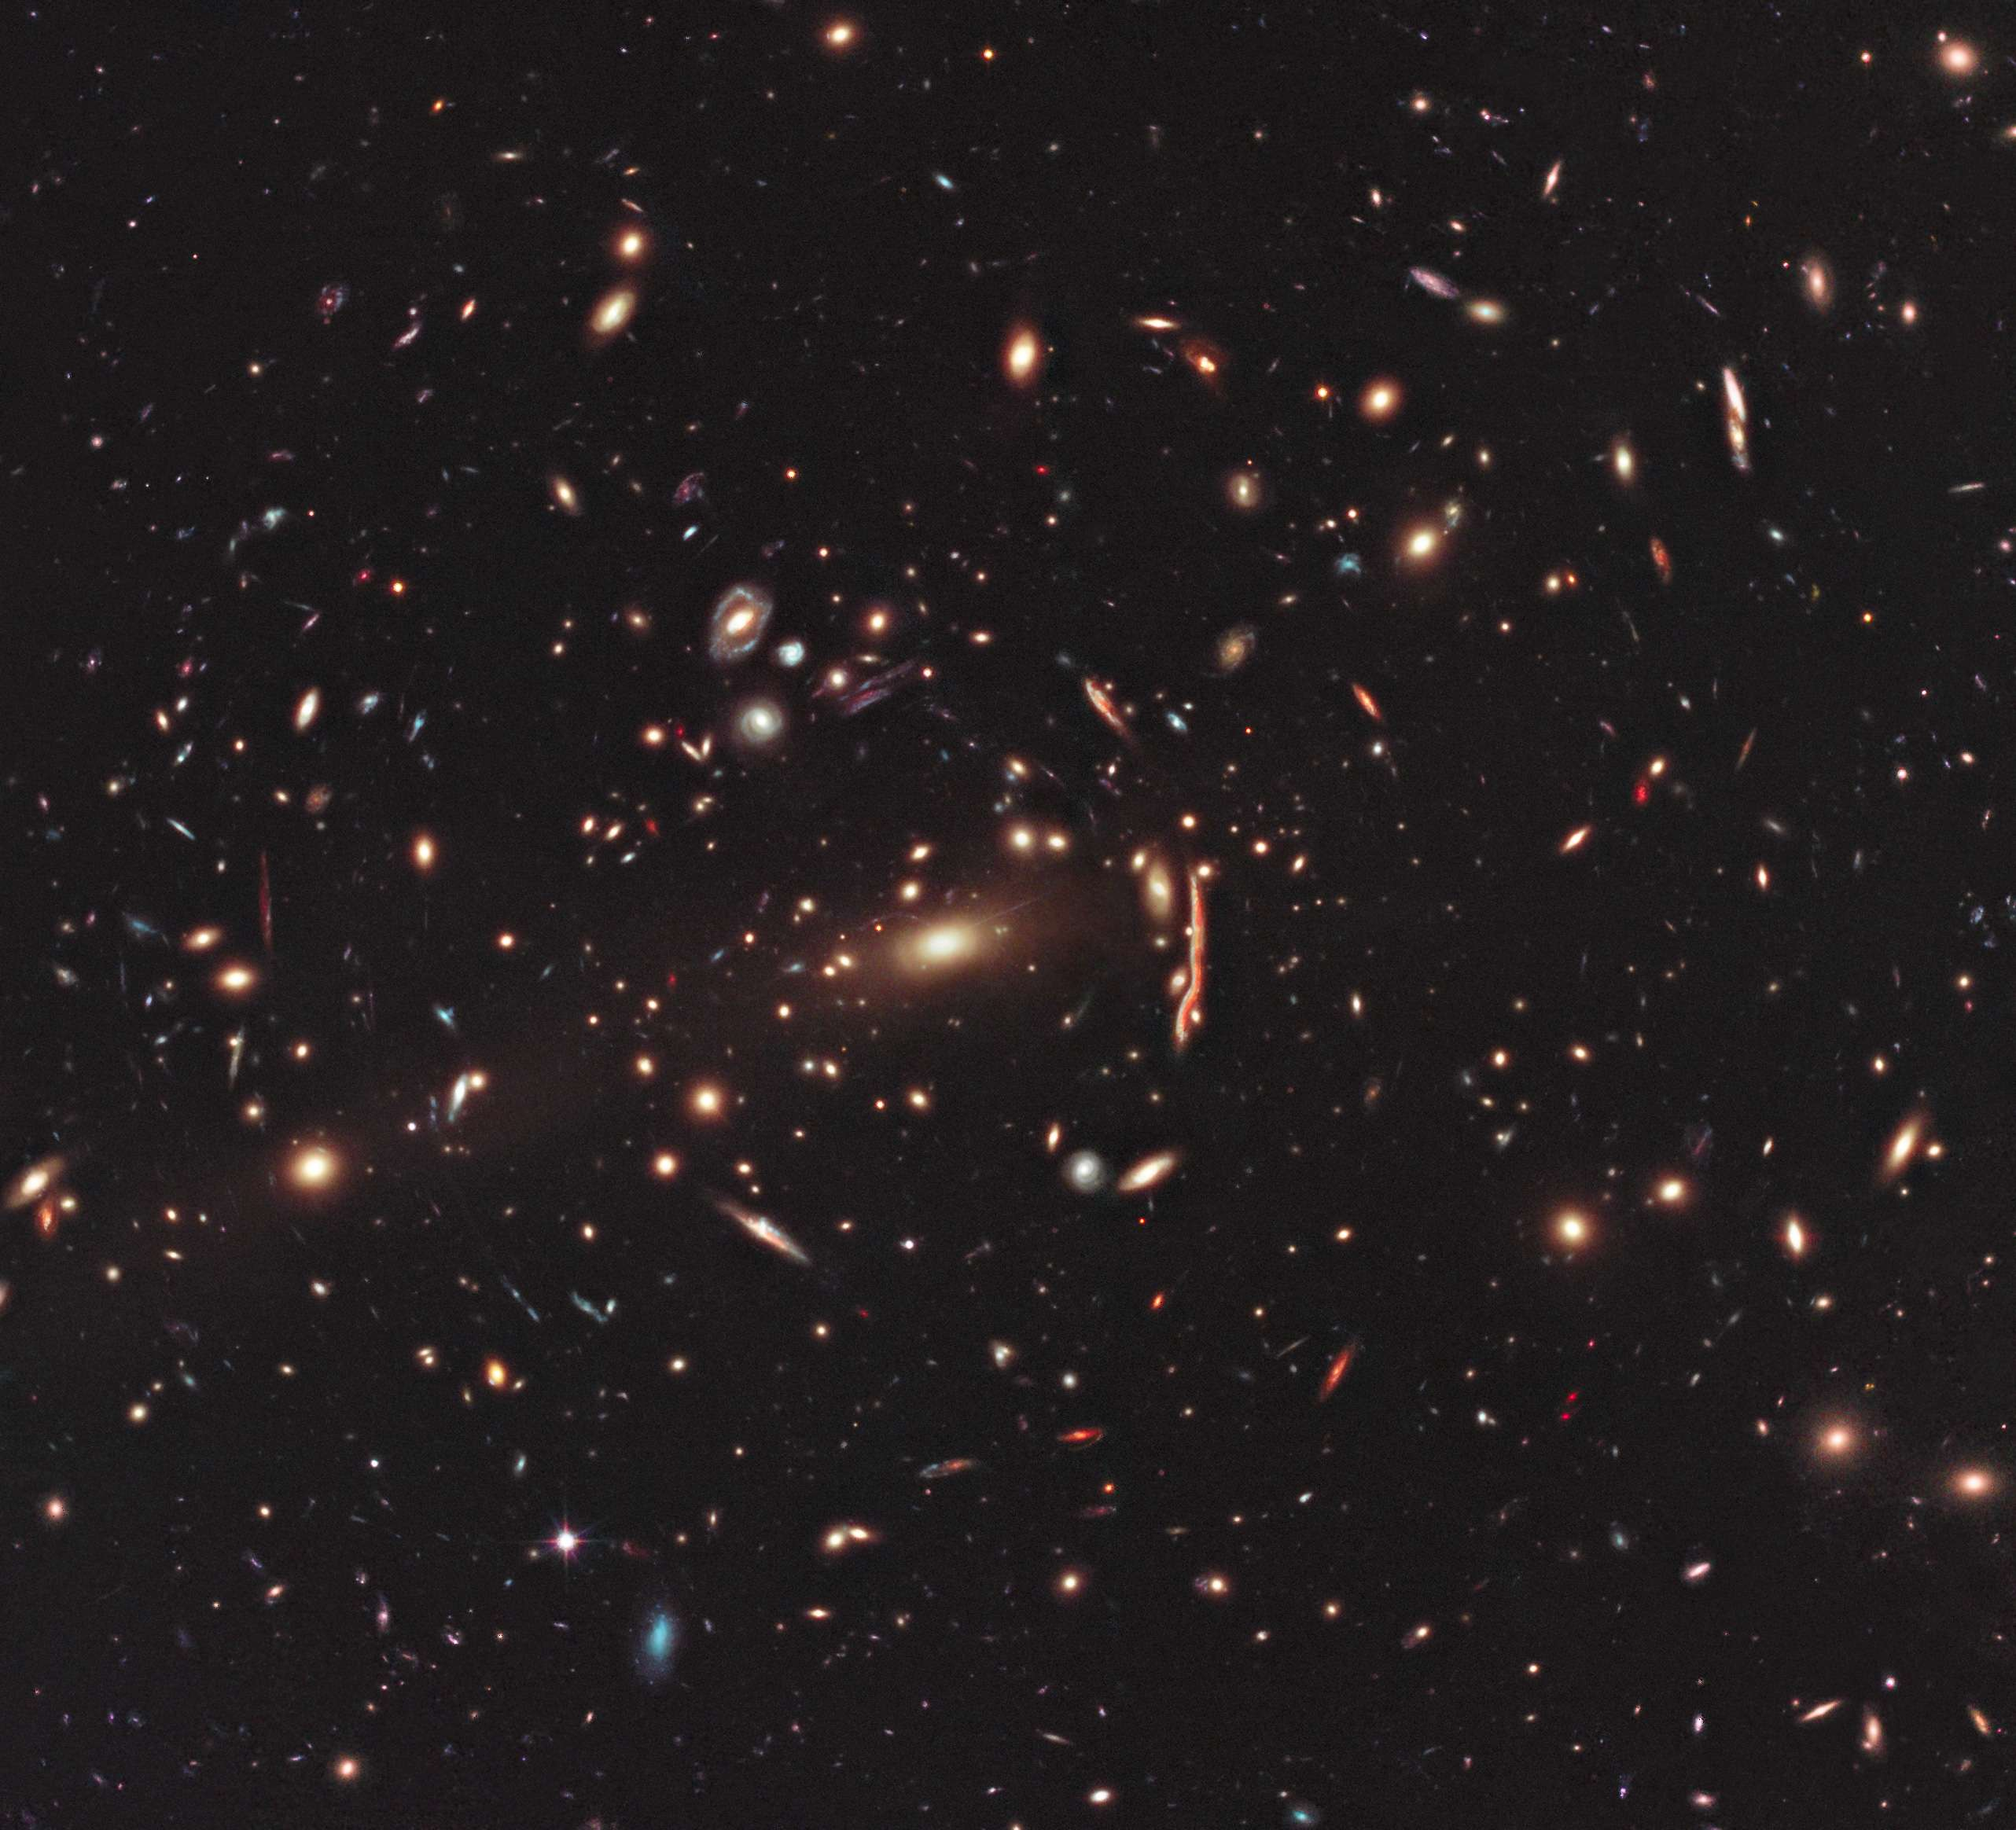
\includegraphics[width=0.6\textwidth]{figures/DMOverview/GravLensIm.jpg}
	\caption[Gravitational lensing by the galaxy cluster MACS J1206.2-0842s.]{Gravitational lensing by the galaxy cluster MACS J1206.2-0842s. The image was taken by the NASA/ESA Hubble Space Telescope, this galaxy is one of 25 clusters being studied as part of the Cluster Lensing and Supernova survey with Hubble programme. Figured reprinted from Ref.~\cite{GravLensPicture}}
	\label{fig:DMOverview/GravLens}
\end{figure}
\begin{figure}[ht!]
	\centering
	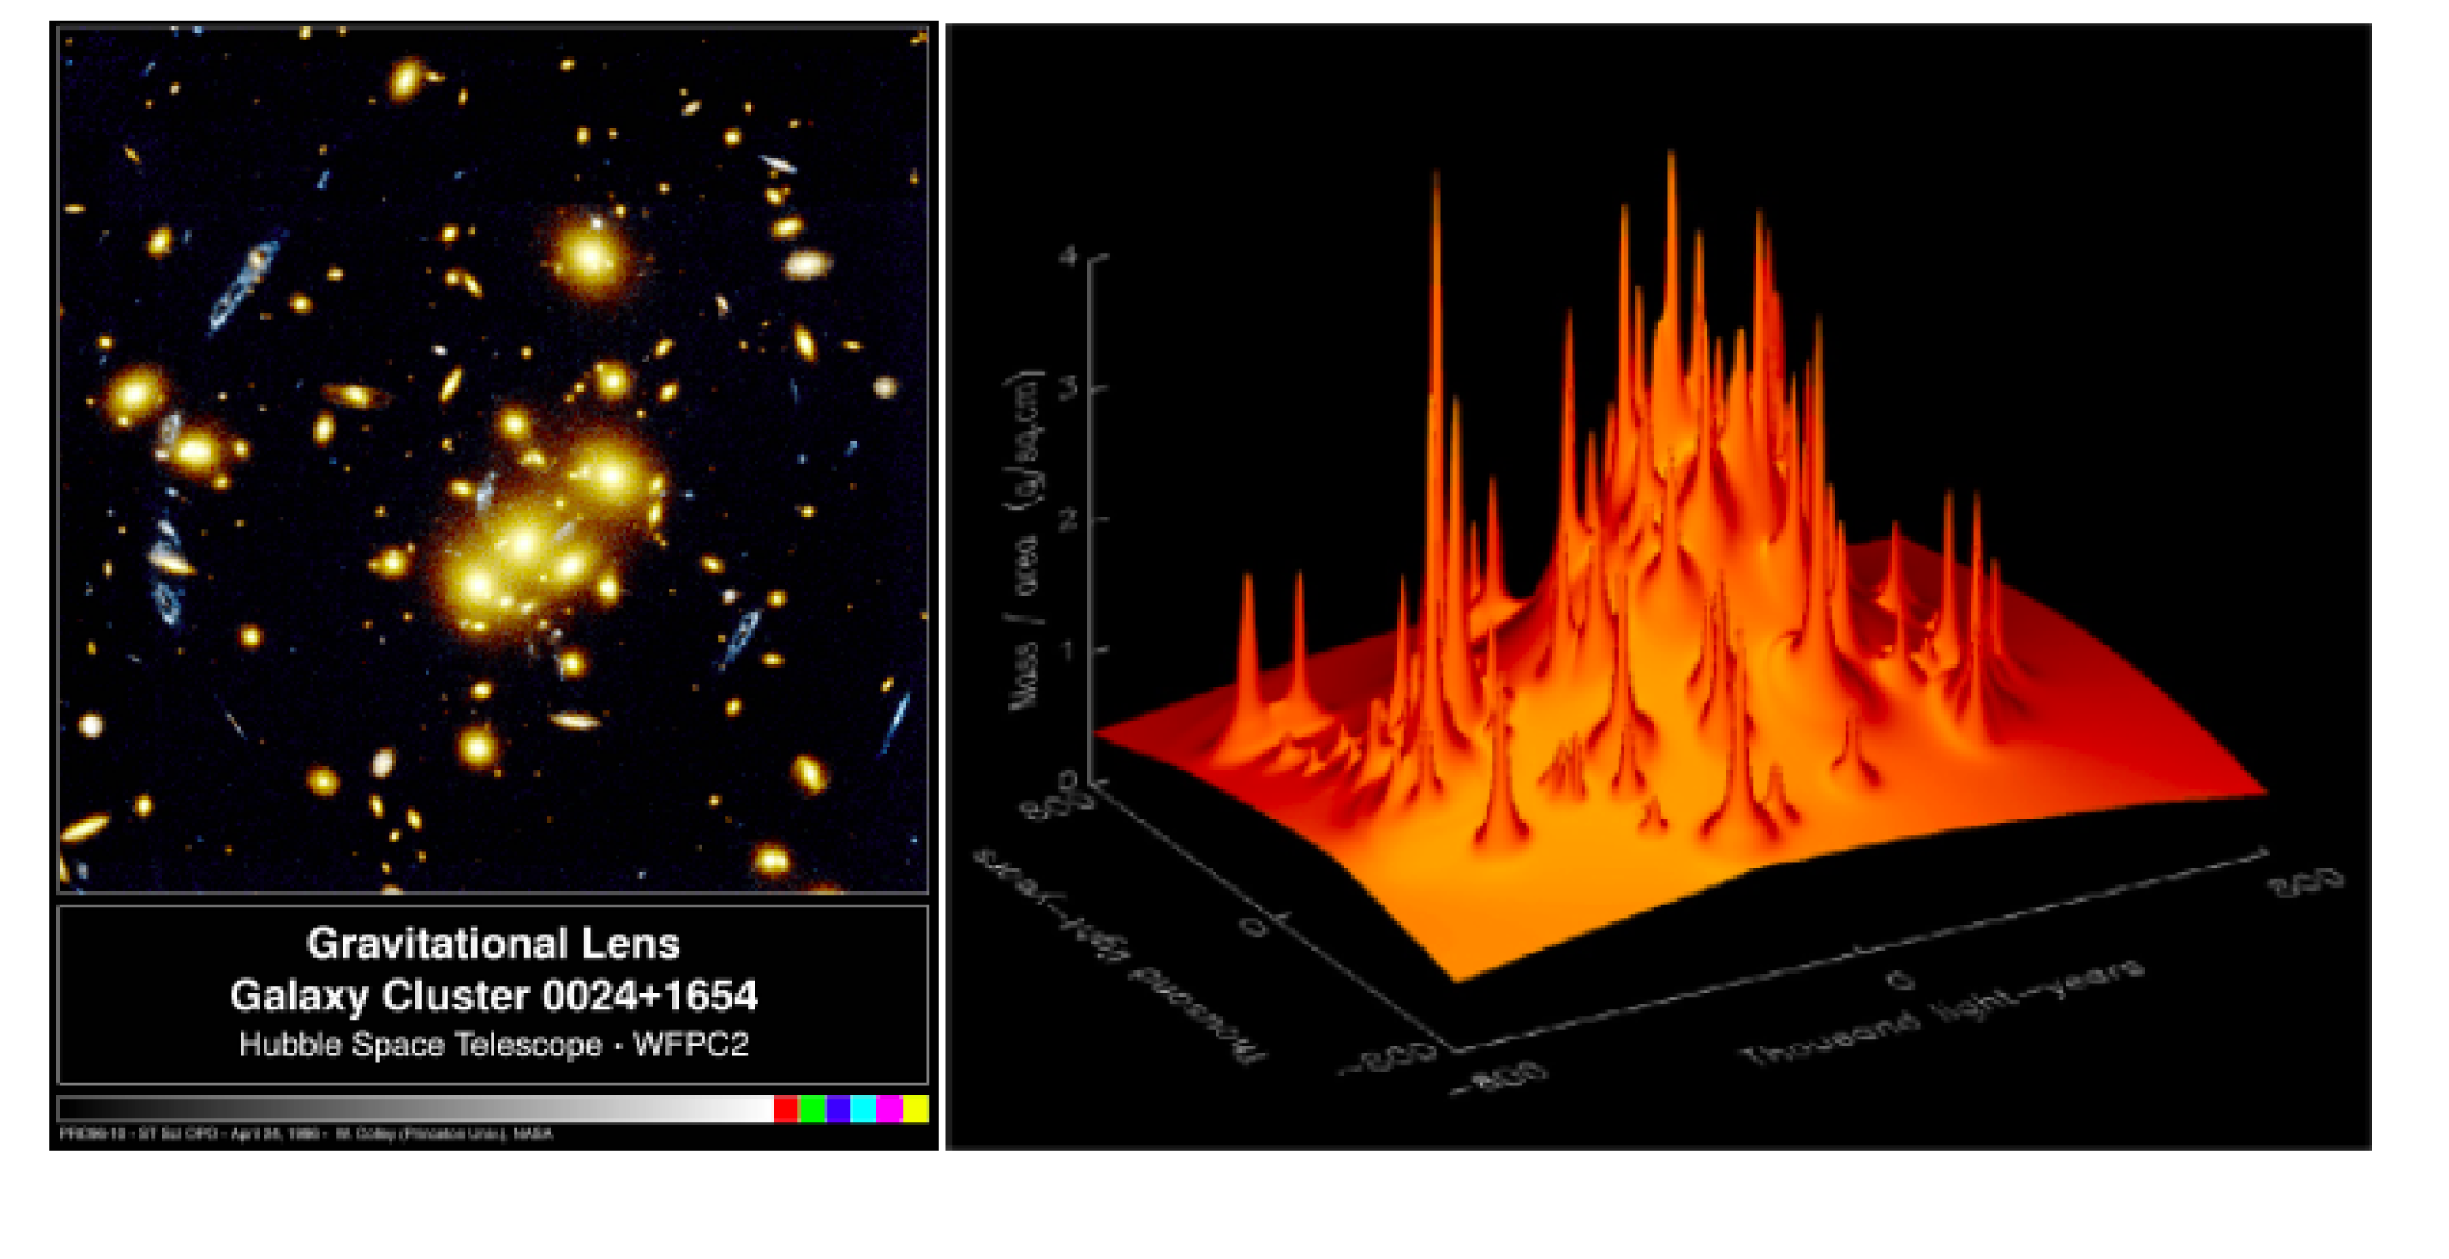
\includegraphics[width=0.8\textwidth]{figures/DMOverview/Strong_Grav_lens.png}
	\caption[\textbf{Left:} Effects of gravitational lensing on multiple galaxies. \textbf{Right:} Reconstruction of gravitational lensing effects.]{\textbf{Left:} An image from the Hubble Space Telescope where the foreground cluster of galaxies gravitationally lenses the blue background galaxy. \textbf{Right:} A reconstruction of gravitational lensing by galaxy cluster. Baryonic matter within the cluster are represented by the sharp spikes and the smooth background component corresponds to some non-visible mass. Figured reprinted from Ref.~\cite{Freese2009}.}
	\label{fig:DMOverview/StrongGravLens}
\end{figure}
\subsubsection{The Bullet Cluster}\label{sec:DMOverview/BulletCluster}
Observations of the Bullet Cluster (1E0657-558) made by the Hubble Space Telescope and the Chandra X-ray Observatory provides evidence towards the existence of dark matter using gravitational lensing.
The Bullet Cluster consists of two galaxy clusters which have collided and are now moving apart. 
%A composite image of the cluster can be seen in \autoref{fig:DMOverview/BulletCluster}, where colour overlays represent the distribution of both luminous and total mass components. The blue regions in the image highlight the total mass distribution derived from gravitational lensing measurements, while the pink regions represent the hot, X-ray-emitting gas that contains the majority of the baryonic matter, such as gas and dust. 
Analysis of the X-ray data found that as the two clusters passed through one another, their gaseous components interacted strongly, colliding, slowing down, and heating up, thus producing intense X-ray emissions. This observation is shown in \autoref{fig:DMOverview/BCXrayData} where X-ray data has the lensing map overlaid.  Whereas measurements made using gravitational lensing indicated that the majority of the non-luminous portion of mass continued without disruption, the spacing between the mass peaks produced with the lensing analysis is shown using green contours in both images in \autoref{fig:DMOverview/BulletCluster}. The lensing mass peaks of the colliding clusters were compared with the X-ray peaks and an offset was found \cite{Clowe_2004}. The offset found between the peaks is considered strong evidence towards the presence of dark matter within the two colliding clusters. Clowe \textit{et al.} applied Modified Theories of Newtonian Dynamics to the results to explain the Bullet Cluster formation but were unable to fully explain the effect where the dark matter component in the regime was equal to the baryonic mass in the system \cite{Clowe2006}. Therefore the presence of dark matter in the cluster still holds true. Thus the Bullet Cluster observations remain as the ``smoking gun'' in the pieces of evidence which support the existence of dark matter in the Universe.
\begin{figure}[ht!]
     \centering
     \begin{subfigure}{0.49\textwidth}
         \centering
         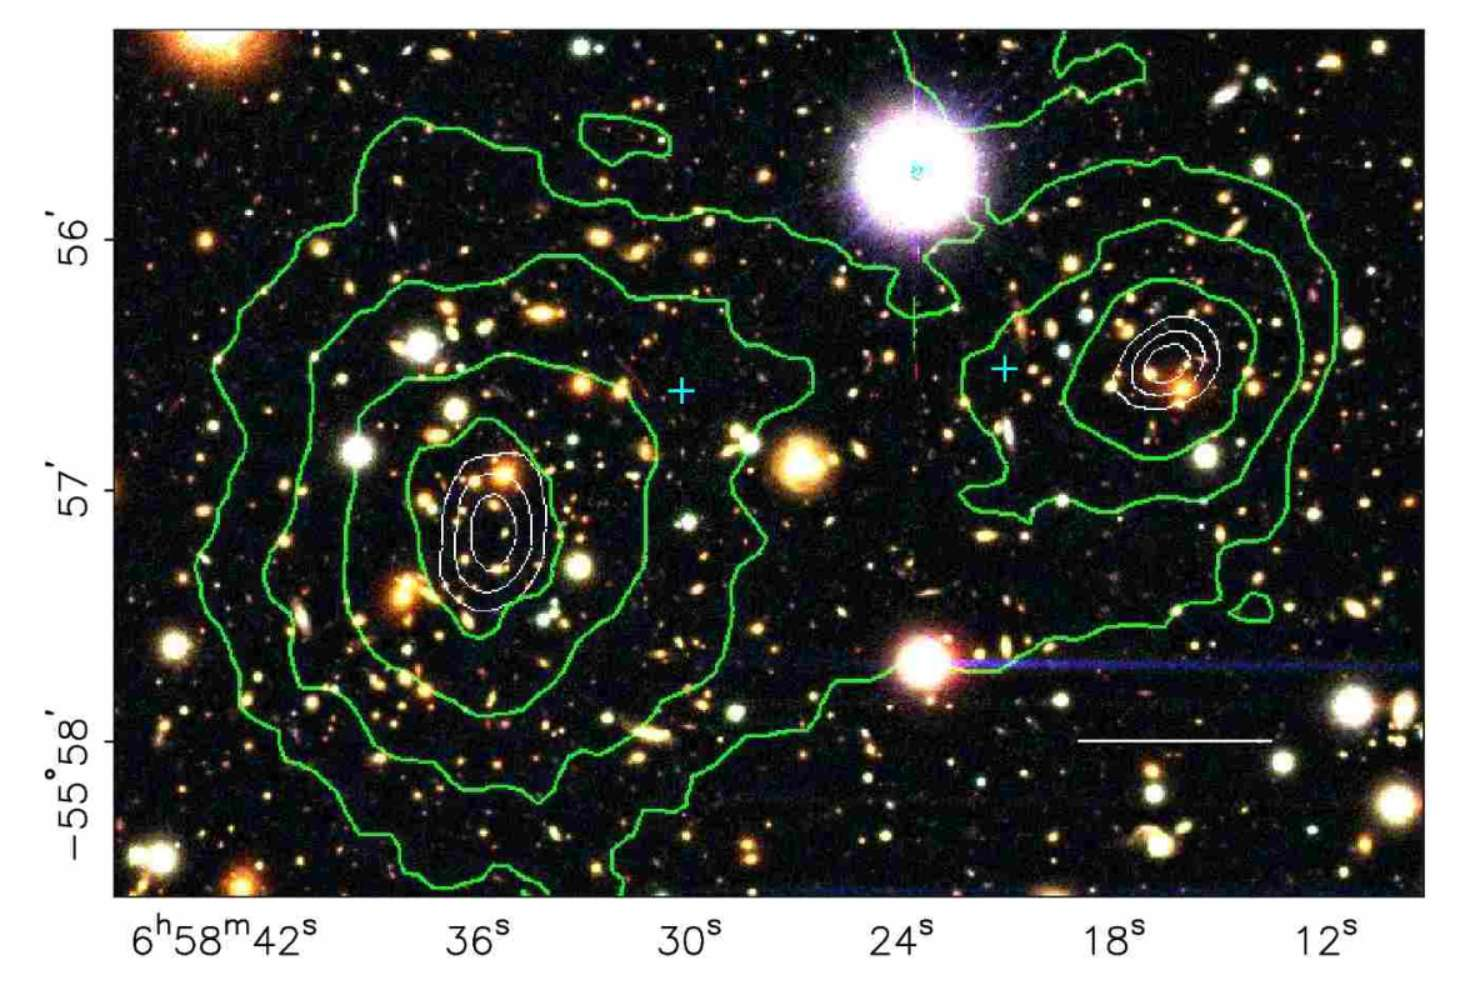
\includegraphics[width=\textwidth]{figures/DMOverview/f1a.new.jpeg2ps.png}
         \caption{}
         \label{fig:DMOverview/BCGravLensMap}
     \end{subfigure}
     \hfill
     \begin{subfigure}{0.49\textwidth}
         \centering
         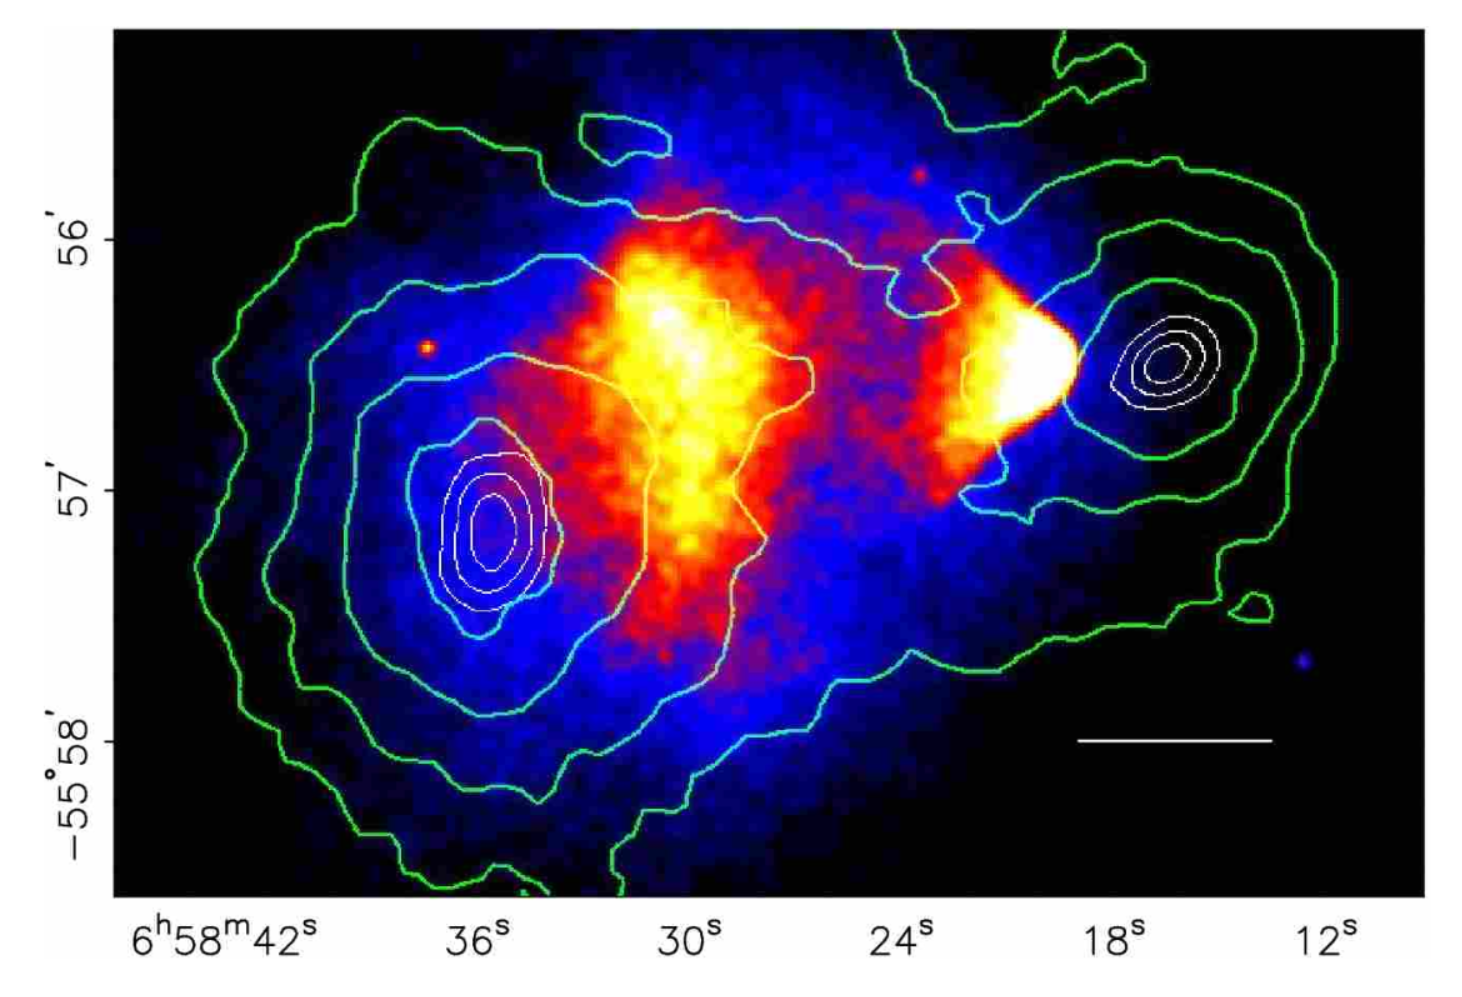
\includegraphics[width=\textwidth]{figures/DMOverview/f1b.new.jpeg2ps.png}
         \caption{}
         \label{fig:DMOverview/BCXrayData}
     \end{subfigure}
     \caption[The Bullet Cluster (1E0657-558) resulting from merger of two galaxy clusters.]{The Bullet Cluster (1E0657-558) resulting from merger of two galaxy clusters. \textbf{Left:}~A colour image from the Magellan images of the merging cluster, the white bar in the lower right of the image indicates 200~kpc at the distance of the cluster. \textbf{Right:}~An image from the Chandra X-ray Observatory. The green contours in both panels indicate the weak lensing reconstruction. Figures reprinted from Ref.~\cite{Clowe2006}.}
     \label{fig:DMOverview/BulletCluster}
\end{figure}

\subsection{The Cosmic Microwave Background}\label{sec:DMOverview/CMB}
The Cosmic Microwave Background (CMB) was first predicted by Ralph Alpher and Robert Herman in 1948 \cite{CMBprediction}, and subsequently discovered by Arno Penzias Robert Woodrow Wilson in 1964 \cite{CMBDisco}. The CMB is relic radiation released after the Big Bang during the recombination epoch. The Universe was filled with an extremely dense, hot-plasma of photons and charge particles. There was an initial rapid expansion of the Universe over 380,000 years until the rate of expansion decreased as the temperature cooled approaching the recombination epoch \cite{DMPrimer}. During this time neutral particles were formed which don't interact with photons. The photons which scattered from free electrons in the plasma state were able to stream freely through the Universe. The CMB is the result of the photons released during this ``last scattering'' \cite{Cirelli:2024ssz}.

The CMB is not completely homogeneous and isotropic, however it can still be viewed as a black body spectrum with a temperature of $(2.726\pm0.001)$~K \cite{Fixsen_2009}. Small fluctuations in the relic density after recombination are echoed in the relic temperature when gravity began to dominate matter. These variations are known as the CMB anisotropy. As a result, the CMB carries an imprint of the presence of dark matter and dark energy which are reflected in acoustic oscillations in the plasma where gravity provided the restoring force. The main observable is the CMB power spectrum shown in \autoref{fig:DMOverview/CMBPowerSpec} which is obtained by performing a spherical harmonic Fourier transform of the CMB temperature shown in \autoref{fig:DMOverview/CMBImg}, and then computing the variance by averaging over the $2l+1$ orientations for each value of the angular momentum $l$ \cite{Cirelli:2024ssz}. The variations are compared to predictions of inflationary Big Bang cosmology which infers information on the contents of the Universe. More precisely, the CMB peaks are due to acoustic oscillations of the baryon/photon fluid. The positions and amplitudes of the peaks represent the relative amount of dark matter with respect to normal matter, where only the latter undergo acoustic oscillations. Global fits to the spectrum find that these oscillations and additional cosmological observations can be well produced by the Standard Model of cosmology which includes dark matter ($\Lambda \text{CDM}$). The x-axis in \autoref{fig:DMOverview/CMBPowerSpec} is a rank of the multiple moment which is inversely proportional to the angular coverage of the sky where,
\begin{equation}
    l \approx\frac{180^{\circ}}{\theta_{res}(degrees)},
\end{equation}
which is treated as a continuous variable \cite{Young2016}. The first peak t $l=200$ infers the total energy-matter density ratio to be $\Omega_{total}=1$. The size and location of the peak relates to the ``flat'' shape of the universe. The second peak centred at $l\approx500$ informs how much baryonic matter is present in the universe. And the third peak at $l\approx700$ describes both the baryonic and dark matter components, where the difference between the second and third peak provides information of the density of dark matter in the early universe \cite{Young2016}.
\begin{figure}[!ht]
     \centering
     \begin{subfigure}{0.47\textwidth}
         \centering
         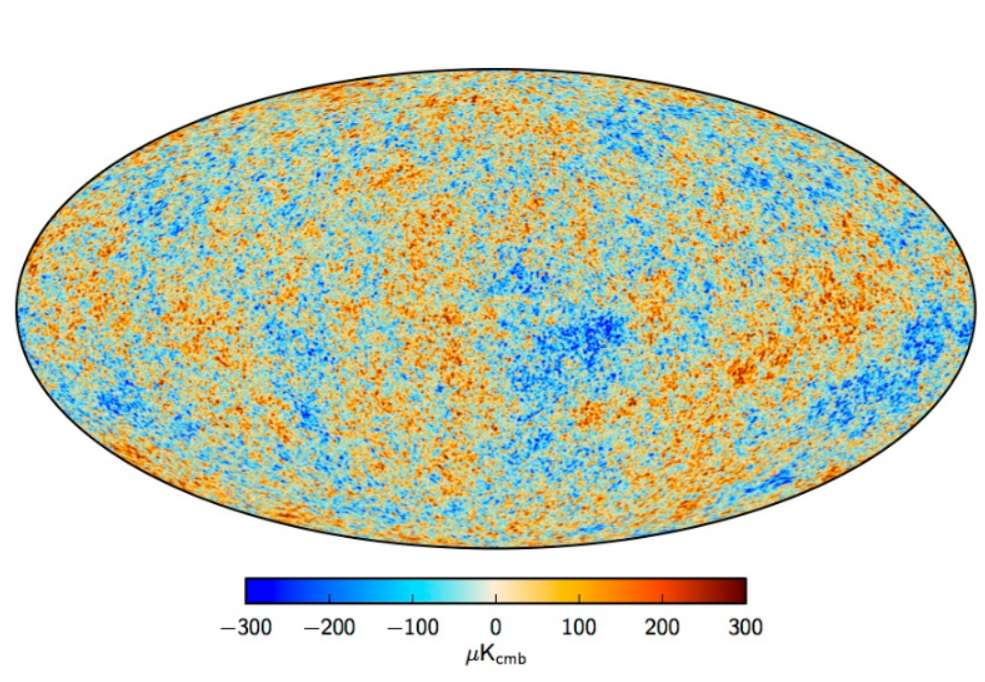
\includegraphics[width=\textwidth]{figures/DMOverview/CMBImg.png}
         \caption{}
         \label{fig:DMOverview/CMBImg}
     \end{subfigure}
     \hfill
     \begin{subfigure}{0.47\textwidth}
         \centering
         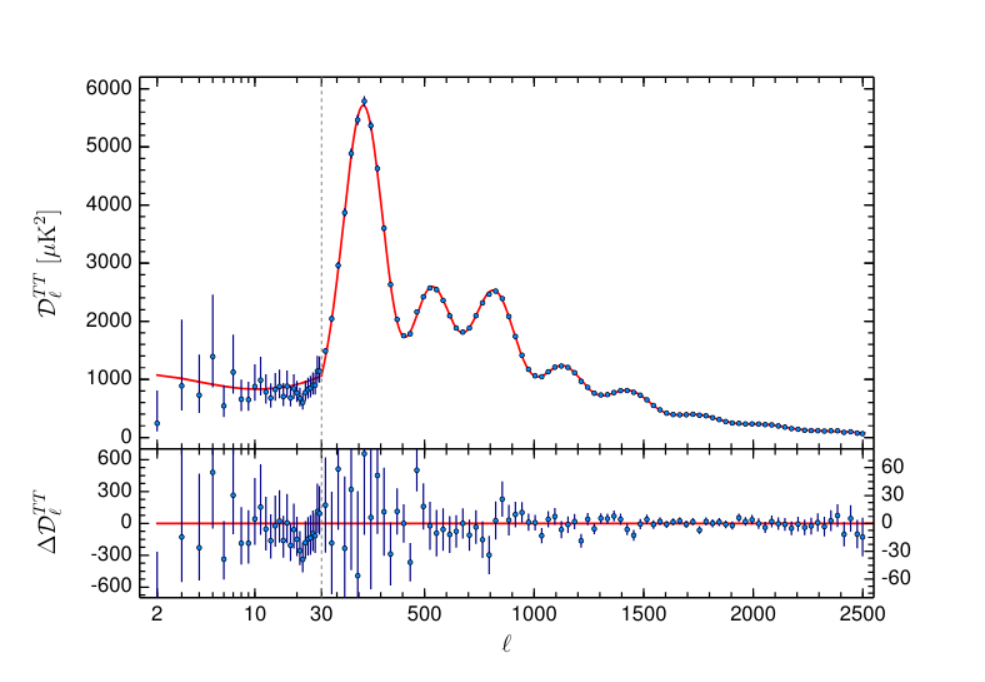
\includegraphics[width=\textwidth]{figures/DMOverview/CMBPS.png}
         \caption{}
         \label{fig:DMOverview/CMBPowerSpec}
     \end{subfigure}
     \caption[The power spectrum of the CMB acoustic peaks is extracted from the map of temperature anisotropies.]{The power spectrum of the CMB acoustic peaks (right) is extracted from the map of temperature anisotropies (left). The data points shown in blue are a collection of measurements taken from Planck, WMAP, ACT and SCP. Figures reprinted from Ref.~\cite{Cirelli:2024ssz}.}
     \label{fig:DMOverview/CMB}
\end{figure}
\subsubsection{$\Lambda$CDM model}\label{sec:DMOverview/LambdaCDM}
The $\Lambda \text{CDM}$ model can be used to show the presence of dark matter in our Universe using the following six parameters: the age of the universe; the density of atoms; the density of matter; the amplitude of the initial fluctuations; the scale dependence of this amplitude; and the epoch of first star formation \cite{LCDMparam}. This model incorporates high-sensitivity small angular resolution measurements in the infrared spectrum from the Planck space observatory \cite{2013Planck}, along with observations of early-universe fluctuations in the Cosmic Microwave Background (CMB) radiation obtained by the Wilkinson Microwave Anisotropy Probe (WMAP) \cite{WMAP}. The data from these sources is shown in \autoref{fig:DMOverview/CMBPowerSpec} where the red line is the fitted $\Lambda \text{CDM}$ model. The most recent estimates from Plank 2018 allow a calculation of the mass-energy distribution in our Universe. The combined analysis results in a spatially-flat universe with a baryon density of $\Omega_{b}=0.049$, a dark matter density of $\Omega_{\text{DM}}=0.265$, and a dark energy density of $\Omega_{\Lambda}=0.686$.

\section{Alternatives to dark matter with the MOND}\label{sec:DMOverview/MOND}
One solution to explain the observations discussed in the proceeding sections is to consider theories based on the Modification of Newtonian Dynamics (MOND). In 1982, Mordehai Milgrom considered the possibility that our understanding of the laws of gravitation on large scales where acceleration is extremely low was wrong and that there was no hidden mass in galaxies \cite{MOND}. A modification of Newtonian dynamics was proposed by Milgrom where the force due to gravity would be scaled by a factor $a_0$ such that, $F=\frac{ma^2}{a_0},$ where $a\ll a_0\sim 1.2\times10^{10}~\text{ms}^{-2}$ \cite{HistoryofDM}. Leading to the following formulation:
\begin{equation}
\begin{split}
    \frac{GMm}{r^2}&=\frac{mv^2}{a_0r^2}\\
    \Rightarrow v^2&=GMa_0
\end{split}
\end{equation}
This formulation states that a galaxy's orbital velocity would not be dependent on the distance from the galactic centre. The flatness seen in galactic rotation curves, shown in \autoref{fig:DMOverview/NGC6503}, could now be explained with the introduction of Milgrom's acceleration constant. However, this initial formulation had theoretical flaws in which momentum, angular momentum and energy were not conserved. Additionally, MOND was not compliant with general relativity, so for MOND to be considered as an alternative to dark matter both the classical and relativistic components needed to be addressed.
Through collaboration with Jacob Bekenstein, the pair attempted to resolve the issues of MOND \cite{Bekenstein1984}. In 2004, Bekenstein proposed a new theory, Tensor-Vector-Scalar
gravity (TeVeS) which would provide a solution to relativistic theories of MOND when applied to gravitational lensing \cite{TeVeS}. TeVeS was considered the leading theory to support MOND but following the discovery of the Bullet Cluster by Clowe \textit{et al.}. 
%The debate that MOND could be a viable solution to explain the observations shifted. 
An $8\sigma$ significance spatial offset of the centre of the total mass from the centre of the baryonic mass peaks could not be explained through modifications of the gravitational force law \cite{Clowe2006}. Many believe that the Bullet Cluster taken together with other increasingly precise cosmological measurements effectively brings the MOND hypothesis to an end \cite{HistoryofDM}. 


\section{Possible candidates for dark matter}\label{sec:DMOverview/Candidates4DM}
The evidence discussed so far in this chapter strongly indicates the existence of non-baryon dark matter in our Universe. Based on early astrophysical observations the new form of matter had to fulfil two criteria, it had to be non-luminous and have mass. But following further observations, physicists postulated that dark matter could arise from some form of undiscovered particle as opposed to some astrophysical material. The new particle should have the following properties:
\begin{itemize}
    \item Stable on timescales of $\mathcal{O}$(14 billion years), timescale of the Universe
    \item Non-baryonic
    \item Very weakly interacting via electromagnetic and strong forces.
    \item Non-relativistic (cold) to allow clustering
    \item Very weak/no self interaction (expect gravitational)
\end{itemize}
A variety of candidates have been proposed ranging in mass from $10^{-22}$~eV to many solar masses \cite{DMPrimer}. The following section will briefly review a small selection of these candidates.
\subsection{Neutrinos}\label{sec:DMOverview/Neutrinos}
One suitable candidate from the Standard Model to be considered as a dark matter candidate would be the neutrino. Being a stable, long-lived and weakly interacting particle, the neutrino seems to fit the requirements outlined above. However, N-body simulations have shown that relativistic neutrinos found in the Standard Model do not allow the structure formation observed in the Universe \cite{White:1983fcs}. The hypothetical, sterile neutrino, proposed to explain the size of the neutrino mass could provide a possible candidate for dark matter. When compared to the `hot' (relativistic) Standard Model neutrino, the sterile neutrino could either be a cold (always non-relativistic) or a warm (only relativistic in the early Universe) dark matter candidate depending on their production mechanise. Thus far experiments have been consistent with the Standard Model \cite{Boyarsky:2018tvu}, but research into this candidate is ongoing as the neutrino sector is probed further \cite{Krasnov:2019kdc}.
\subsection{Axions}\label{sec:DMOverview/Axions}
As well as neutrinos, axions are another form of particle which would be a candidate to solve the dark matter problem. The axion was first postulated to solve the ``strong CP problem'' in 1977 \cite{ConsvCP} due to the CP violation from the experimental bound on the neutrino dipole moment in quantum chromodynamics \cite{Hook:2018dlk}. Currently constraints have been made on the possible axion dark matter mass to be between $10^{-6}$ and $10^{-2}$~eV \cite{Duffy:2009ig}. Experimental searches for the axion are ongoing through photon coupling \cite{ADMX:2018gho,JacksonKimball:2017elr}. {\color{red} BP: Maybe explain a bit: why EM coupling, ADMX, behaves like a field}
\subsection{MACHOs}\label{sec:DMOverview/MACHOs}
A candidate at the other end of the mass scale could be Massive Astrophysical Compact Halo Objects (MACHOs) which emit little to no radiation. MACHOs could come in the form of neutron stars, black
holes, brown dwarfs or un-associated planets which could be used to explain the discrepancies observed in the cosmological observations discussed above. However, studies have shown that the majority of the dark matter density cannot entirely comprise of MACHOs \cite{Becker:2004ni,MicroLens}. Through a search for microlensing\footnote{Microlensing is a form of gravitational lensing which produces very small angular separations between the multiple images or changes in brightness and the image they produce is too small to be resolved.} in the Large Magellanic Cloud (LMC), the MACHO Project found that MACHOs would constitute only $8~\%$ of the dark matter halo in the LMC. This result ruled out a $100\%$ MACHO halo model \cite{MicroLens}.
The baryonic nature of the MACHOs additionally impose constraints on their contribution to the total baryonic density observed through cosmological measurements and thus cannot be used exclusively explain the mass-energy distributions in the Universe \cite{Planck2018}.

\subsection{WIMPs}\label{sec:DMOverview/WIMPs}
Weakly Interacting Massive Particles (WIMPs) is the final candidate to be discussed in this work and are well motivated and the more widely excepted candidates for dark matter. They are proposed as non-relativistic, heavy particles with interaction strengths on the scale of the weak force. The current dark matter density can be reproduced with the presence of WIMPs in the cosmological argument, this is known as the `WIMP miracle'\cite{DMPrimer}. Whilst the early universe was in a hot dense state, WIMPs were in thermal equilibrium with the cosmic plasma. During this time the annihilation rates of WIMPs producing Standard Model particles and the reverse process was in equilibrium. During the expansion of the Universe  the temperature of the plasma cooled below that of the WIMP mass which led to the decoupling of WIMPs and baryonic matter \cite{DMProd}. During this time the production of WIMPs from Standard Model particles was suppressed, as such the WIMP density decreased exponentially with temperature. The dark matter relic density was reached when the annihilation rate of WIMPs became less that the Hubble expansion rate. Thus the cross-section required to detect a particle in the current density is of order of the weak interaction scale \cite{DMProd}.

\begin{flushleft}
The candidates discussed in the sections above were not originally proposed to solve the dark matter problem, but were proposed to provide solutions to other models and theories in physics. The external motivation only strengthens the importance of the candidates.
\end{flushleft}

\section{Searching for dark matter}\label{sec:DMOverview/DetectionOfDM}
The particle dark matter hypothesis can be tested via the following three mechanisms: production at particle accelerators; indirect detection by searching for signals from annihilation products; and direct detection via scattering on target nuclei. The possible dark matter, $\chi$, coupling to a standard model particle, P, is shown in \autoref{fig:DMOverview/detection_schem}. The following sections will review the different mechanisms as well as the current status of the searches so far. 
\begin{figure}[ht!]
	\centering
	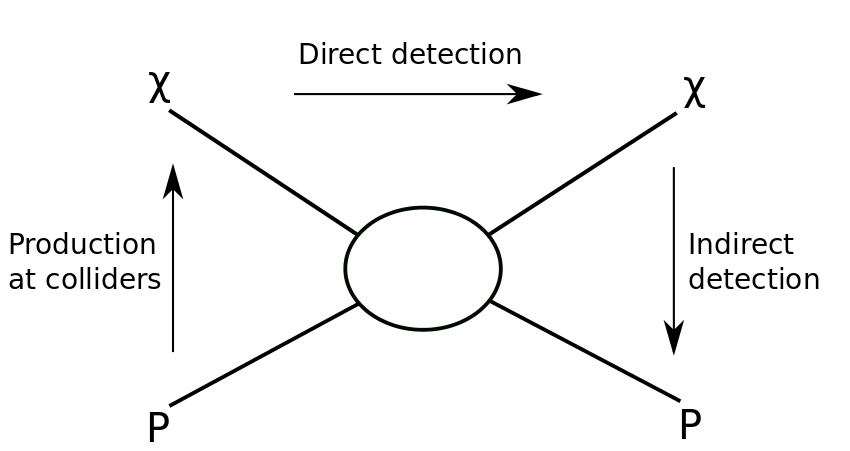
\includegraphics[width=0.7\linewidth]{figures/DMOverview/Detection_schematic.png}
	\caption[Schematic illustrating the possible dark matter detection methods.]{Schematic illustrating the three possible dark matter detection methods. Figured reprinted from Ref.~\cite{DirectDetection2015}.}
	\label{fig:DMOverview/detection_schem}
\end{figure}
\subsection{Dark matter production at particle colliders}\label{sec:DMOverview/DMProdColliders}
The production of dark matter, namely WIMPs, at particle colliders is a well motivated approach as the electroweak scale is powerfully probed by colliders such as Large Hadron Collider (LHC) at CERN \cite{Evans:2008zzb}. Since the start of the LHC in 2008, the ATLAS \cite{ATLAS:2008xda} and CMS \cite{CMS:2008xjf} experiments have searched for new particles in proton-proton collisions with a centre-of-mass-energy of 7~TeV to 13~TeV. Besides the discovery of the Higgs boson \cite{ATLAS:2012yve,CMS:2012qbp}, ATLAS and CMS experiments searched for new particles by scanning parameter space of different models of new physics such as supersymmetry \cite{hteagle:thesis}. 

Collider searches for dark matter can generally be divided into two categories: those that involve dark matter particles in the final state and those that do not. Both cases are dependent on the mass of the dark matter particle, $\chi$, and the mass of the mediator which can be a known Standard Model (SM) particle (often but not exclusively the Higgs Boson) or an exotic mediator particle \cite{Penning:2017tmb}. 

If the dark matter particle mass is less than the mediator, then a WIMP pair is produced in the direction opposite to that of the visible particles. This results in a characteristic `mono-$X$' signature, where the `missing transverse energy', or more correctly `missing transverse momentum', ($E^{\text{miss}}_\text{T}$) and the visible particles $X$ are nearly back-to-back. The particle produced in this collision can be a multitude of particles such as $\gamma, q, g, W, Z, H$ and others. This mechanism is more commonly referred to as collider based dark matter production. An example event from a mono-$X$ search is shown in \autoref{fig:DMOverview/Mono-XEventViewer}.

\begin{figure}[ht!]
    \centering
    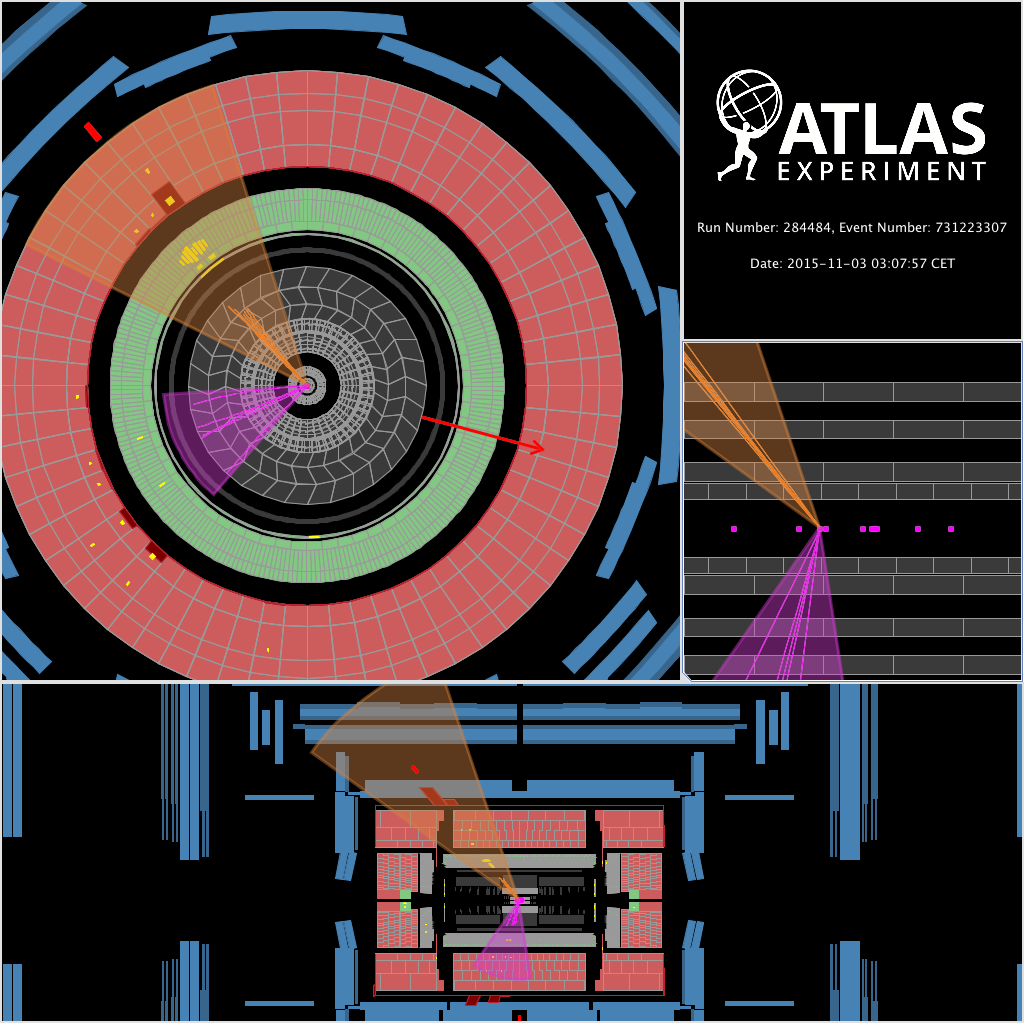
\includegraphics[width=0.65\linewidth]{figures/DMOverview/MonoXEventViewer.png}
    \caption[An event from a Mono-Higgs search from the ATLAS detector at the LHC.]{An event from a Mono-Higgs search from the ATLAS detector at the LHC. This event is characterized by $E^{\text{miss}}_\text{T}$~=~213~GeV (direction indicated with the red arrow) and two $b$-tagged small-R calorimeter jets that form a dijet system with $m_{jj}~=~120~\text{GeV}$ (shown in orange and magenta). Figure reprinted from Ref.~\cite{ATLAS:2016btj}}
    \label{fig:DMOverview/Mono-XEventViewer}
\end{figure}

If the mediator is lighter than the dark matter, then the mediator becomes off-shell, then the processes proceeds via a virtual exchange and the process is suppressed. This is considered a search for a beyond the SM mediator \cite{hteagle:thesis}. If the hypothetical mediators couple to SM particles and the collider is powerful enough then the mediator could be produced in the annihilation of SM particles.  An example is the dijet analysis
looking for a narrow peak in the invariant mass of the two jets, $m_{jj}$ \cite{Penning:2017tmb}.
So far results remain consistent with Standard Model expectations \cite{CMS:2017jdm,ATLAS:2016bek} and significant constraints on a number of dark matter models and masses have been made, the mass reach that the CMS experiment has achieved is shown in \autoref{fig:CMS-MassReach}.

\begin{figure}[ht!]
    \centering
    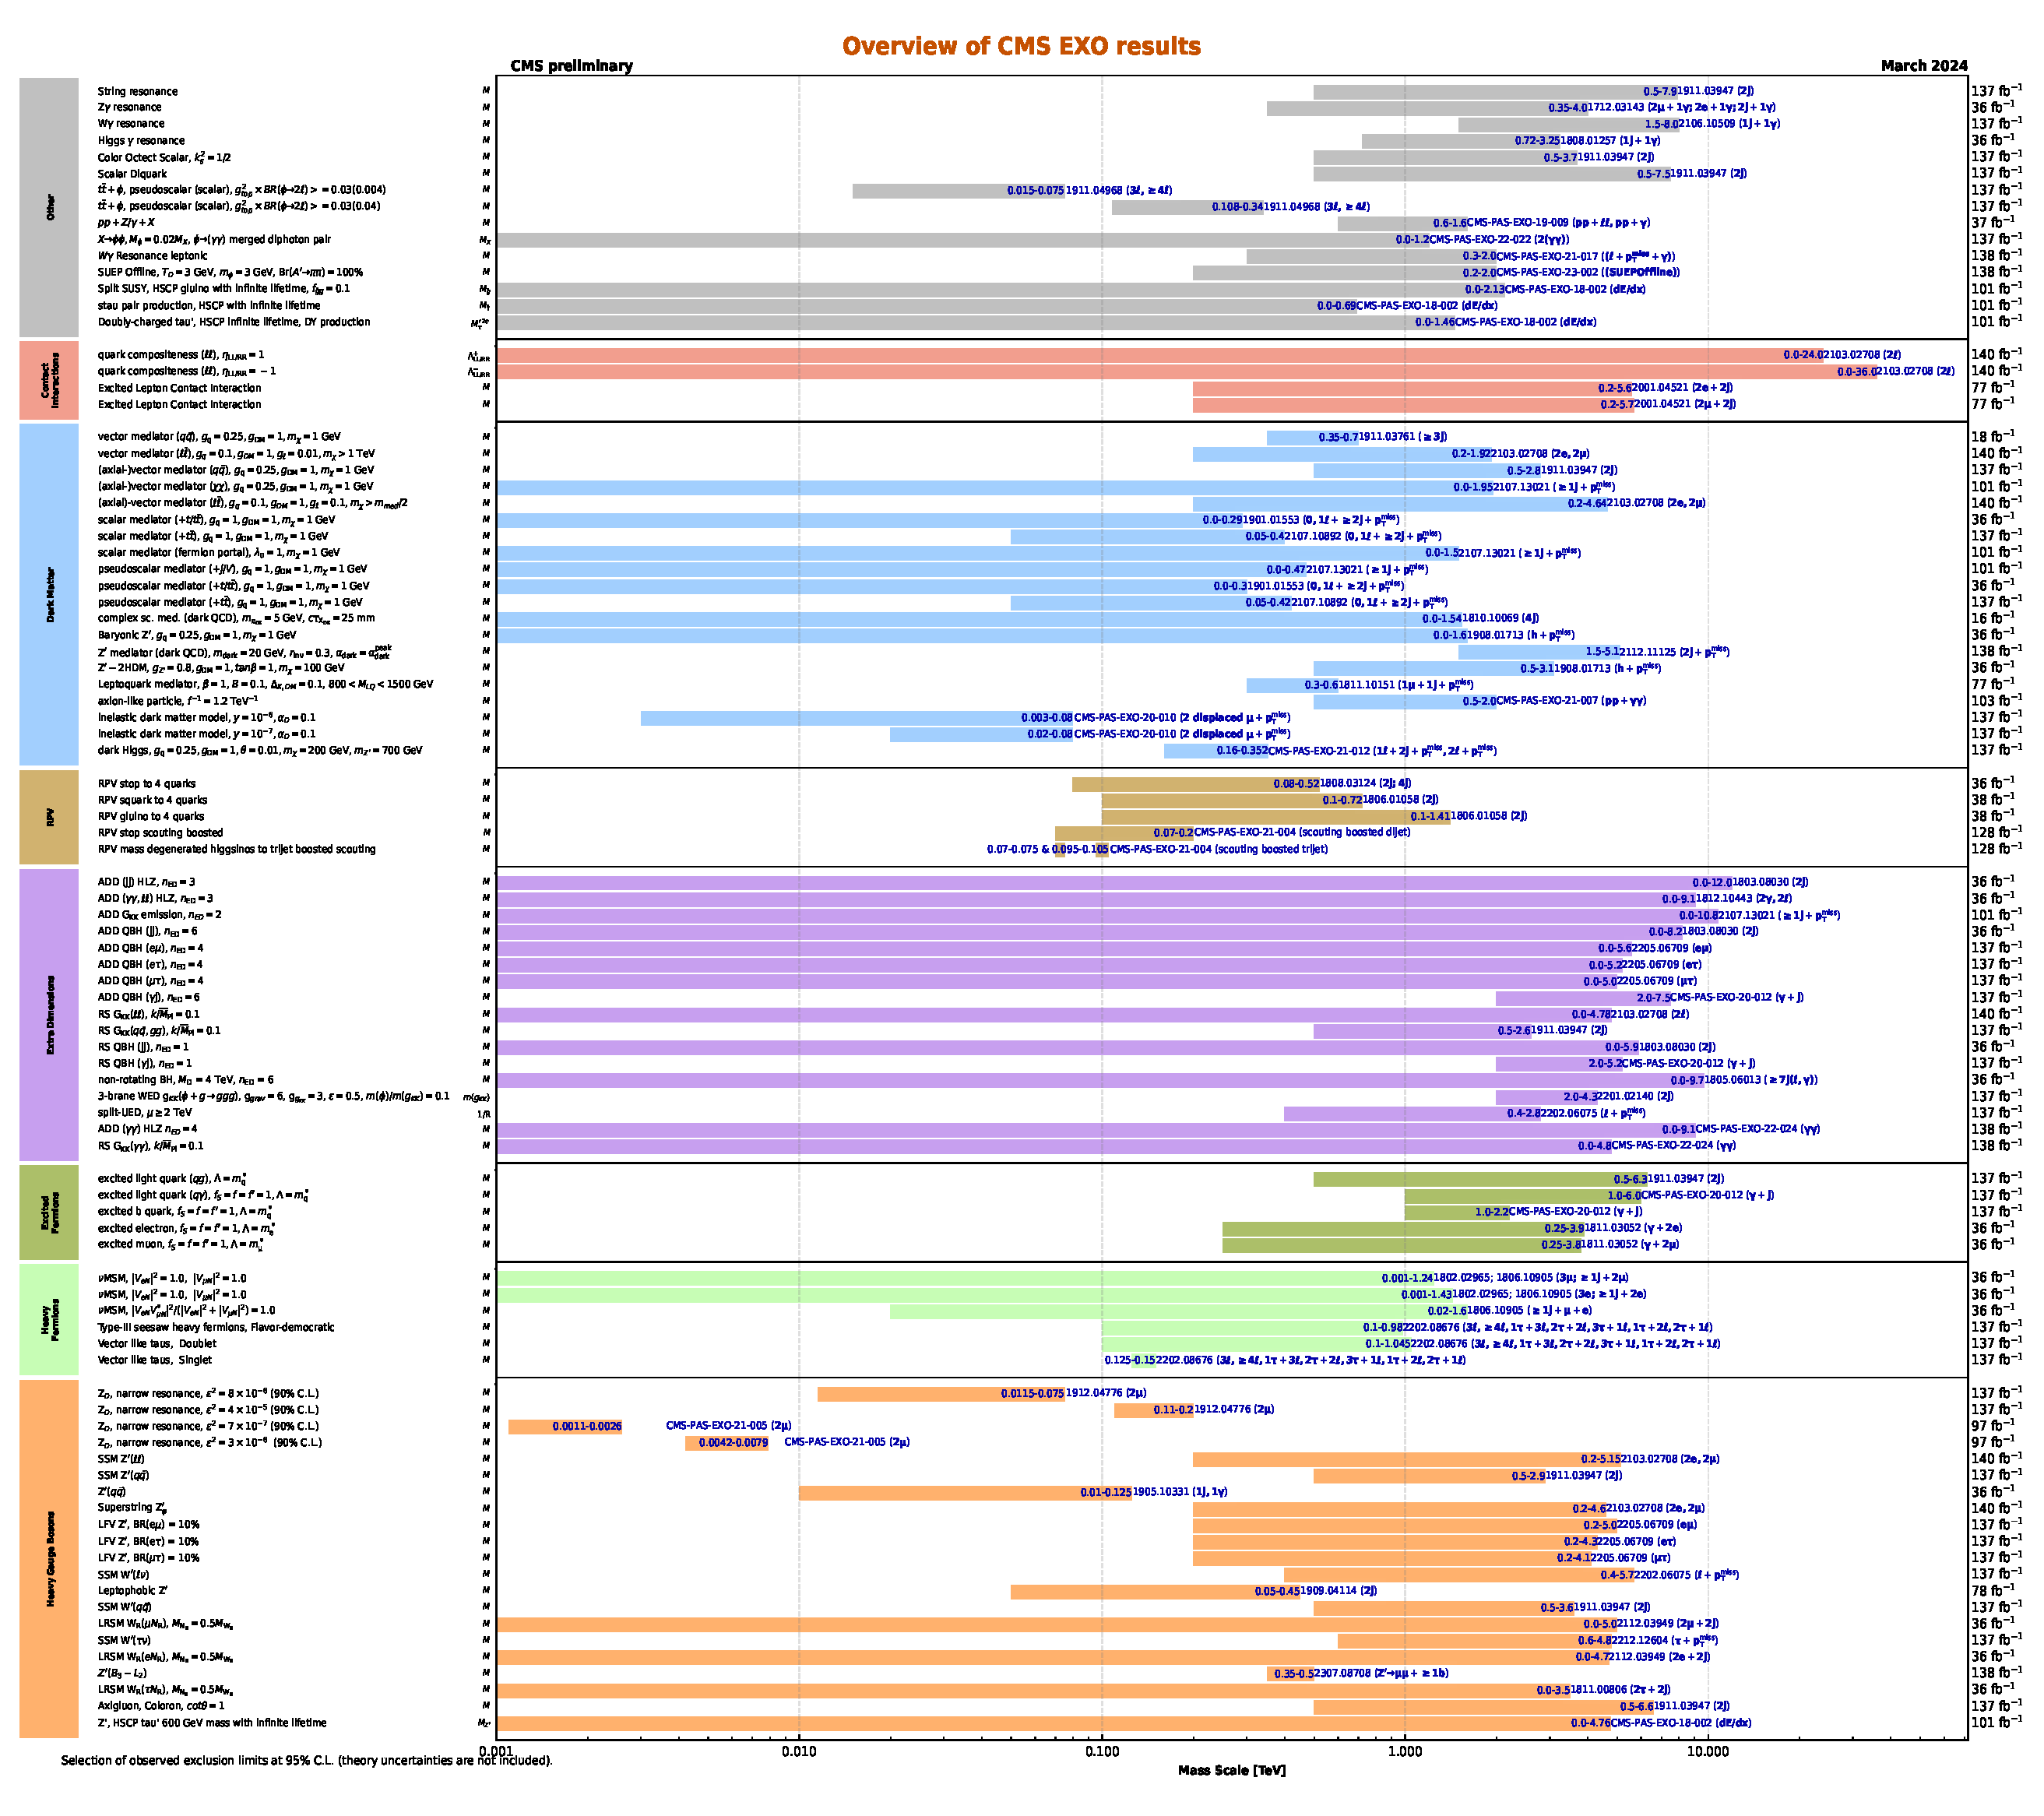
\includegraphics[width=0.9\linewidth]{figures/DMOverview/CurrentBarChartVersion_v14.pdf}
    \caption[A bar chart representing an overview of the mass reach of CMS analyses.]{A bar chart representing an overview of the mass reach of CMS Exotica analyses for the 13~TeV data \cite{CMS-MassReach}.}
    \label{fig:CMS-MassReach}
\end{figure}

Dark matter searches at colliders are not restricted to the two mechanisms outlined above, some of which include long-lived particle searches \cite{Mitsou:2021tti}, new signatures and production modes \cite{Dienes:2021cxr,tcarter:thesis}, dark sectors searches \cite{Cohen:2017pzm,ajaspan:thesis}, novel instrumentation and different beams \cite{Feng:2017uoz,Batell:2014mga}. The collider will play a crucial role in case a discovery takes place first in either direct or indirect searches as they will be well suited to produce and measured dark matter under laboratory conditions.

\iffalse
Besides the discovery of the Higgs boson \cite{ATLAS:2012yve,CMS:2012qbp}, ATLAS and CMS experiments searched for new particles by scanning parameter space of different models of new physics such as supersymmetry \cite{hteagle:thesis,tcarter:thesis,ajaspan:thesis}. To infer the production of a dark matter particle at a collider, events with missing transverse momentum or energy would first need to be observed.  This mechanism is described in the following:
\begin{equation}
    pp\rightarrow \chi \overline{\chi}+x,
\end{equation}
where $p$ represents a proton, $x$ represents a hadronic jet, a photon or a leptonically decaying Z or W boson \cite{DirectDetection2015}. So far results remain consistent with Standard Model expectations \cite{CMS:2017jdm,ATLAS:2016bek} but further searches are ongoing.
\fi

\subsection{Indirect detection of dark matter}\label{sec:DMOverview/IndirectDM}
Based on evidence from observational cosmology, dark matter can gravitationally accumulate in halos around astronomical objects such as stars, galaxies, our Sun and our galactic centre. These sources are therefore possible regions in which to conduct indirect dark matter searches. The increased dark matter density in these regions could produce a measurable particle flux of dark matter particles self-annihilating, scatter, or decay into Standard Model particles \cite{Strigari:2012acq}. The search for such signals is denoted as `indirect detection'. Examples of possible annihilation channels are:
\begin{equation}
    \chi\overline{\chi}\rightarrow\gamma\gamma,\gamma Z,\gamma H\quad\text{or,}
\end{equation}
\begin{equation}
    \chi\overline{\chi}\rightarrow q\overline{q},\,W^+W^-,\,ZZ,
\end{equation}
some of the products decay further in $e^-e^+,\,p\overline{p},\,\gamma\text{-rays}$ and neutrinos \cite{DirectDetection2015}. There are many possible indirect detection mechanisms which can be searched for such as observing high energy $\gamma$-rays using atmospheric Cherenkov telescopes which are point specifically in the direction of objects where large amounts of dark matter is expected. The FERMI-LAT collaboration have reported an excess of $\gamma$-rays from the galactic centre of the Milky Way \cite{Fermi-LAT:2015sau}, however it is unclear if the excess signal is from from dark matter annihilations or point source backgrounds \cite{Boyarsky_2011}. However, FERMI-LAT data has be used to publish constraints of dark matter annihilation cross-section from a null result of a dwarf galaxy search \cite{Fermi-LAT:2015ycq}. Additional upper limits have been derived by a number of telescopes \cite{Aleksic:2013xea,HESS:2014zqa,VERITAS:2017tif}. Large neutrino detectors such as ANTARES \cite{ANTARES:2016xuh} and IceCube \cite{IceCube:2009iyf} are able to search for dark matter annihilation into neutrinos. Both experiments have placed constraints on spin-dependent WIMP-proton cross-section. The mechanism considered is that WIMPs scatter off protons in the Sun which results in a sufficient momentum reduction to be bound by the Sun's gravity. The WIMPs bound in this way would then result in the WIMP annihilation to neutrinos more frequently, in addition to other SM particles. The neutrinos produced via this mechanism are expected to have an order of magnitude higher energy than solar neutrinos \cite{Hooper:2025ohk,Super-Kamiokande:2020sgt}.

\subsection{Direct detection of dark matter}\label{sec:DMOverview/DirectDetection}
The direct detection of dark matter aims to observe nuclear or electronic recoils resulting from interactions between the dark matter particle and the target material within a detector. These interactions are expected to produce recoil energies in the range of $1-100\,\mathrm{keV}$, assuming incident dark matter particles with masses between $10-1000\,\mathrm{GeV}/c^2$~\cite{DirectDetection2015}. The resulting signals from such recoils can be observed in one or more of three forms: phonons (heat), ionization (charge), and scintillation (light). Detectors are therefore typically designed to be sensitive to one or two of these signal channels, depending on the detection strategy employed. A schematic representation of this detection process is shown in \autoref{fig:DMOverview/DirectDetectorTriangle} and each of the different direct detection technologies are outlined below:
\begin{figure}[ht!]
	\centering
	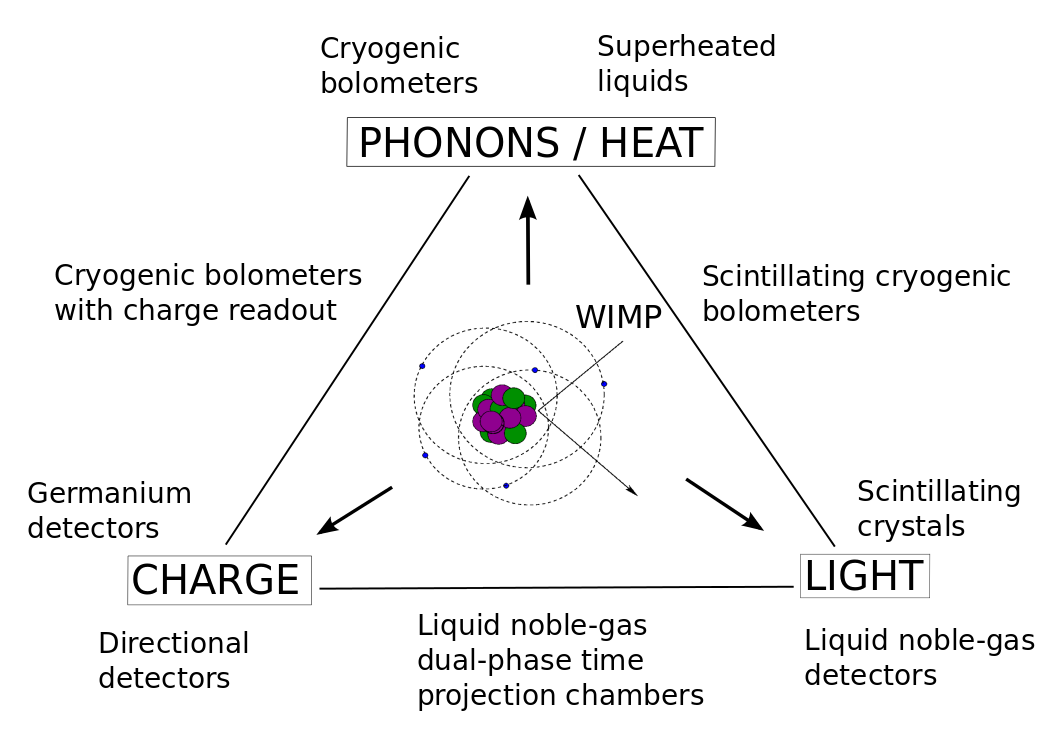
\includegraphics[width=0.6\textwidth]{figures/DMOverview/Direct_direction.png}
	\caption[A schematic showing the possible direct detection signals with corresponding experiments.]{A schematic showing the possible direct detection signals and the corresponding experiments used to observe such signals \cite{DirectDetection2015}.}
	\label{fig:DMOverview/DirectDetectorTriangle}
\end{figure}
\begin{itemize}
    \item \textbf{Anorganic Crystal Detectors} use $\mathcal{O}(1)$kg-scale arrays of high-purity scintillator crystals, mainly NaI(Tl) but also CsI(Tl), which are monitored by low-background photomultiplier tubes (PMTs), shown schematically in \autoref{fig:DMOverview/crystal}. The high mass numbers of I ($A=127$) and Cs ($A=133$) lead to a high sensitivity to spin-independent interactions \cite{Schumann:2019eaa}. However, they lack position reconstruction capabilities, which prevents fiducialisation discrimination and results in relatively high background levels. Consequently, WIMP searches using this technology focus on detecting annual modulations in low-energy signals, which arise from the Earth’s changing velocity relative to the Solar System's motion through the Dark Matter halo. Experiments which rely on this type of detector technology include DAMA/LIBRA \cite{DAMA:2008jlt}, COSINE-100 \cite{COSINE-100:2019lgn} and DAMIC \cite{Privitera:2024tpq}.
    
    \item \textbf{Cryogenic Crystal Detectors} operate via the detection of the heat signal in the form of phonons is measured through the increase in temperature following a particle interaction within the crystalline detector. The sensitivity to record the increase in temperature from an energy deposit is dependent on the detector's heat capacity and how well thermally coupled the detector to the heat bath. These detectors are operated at cryogenic temperatures (typically $\leq50~\text{mK}$) to minimize thermal noise and enhance sensitivity. Dielectric crystals such as Ge and Si are particularly well-suited for cryogenic operation as their heat capacity is given by $C \propto M \times T^3$ below their Debye temperature which is well above room temperature for Ge and Si, where $M$ denotes the mass of the detector \cite{Schumann:2019eaa}. Transition Edge Sensors (TES) are used to detect the tiny temperature rise. The TES is operated at the transition temperature between their super-conducting and the normal-conducting state where a small change in temperature will result in a large change in resistivity of the wire and subsequent current flowing through the wire in contact with the crystal. An alternative detector-type are neutron transmutation doped (NTD) germanium thermistors whose resistivity strongly depends on the temperature \cite{Schumann:2019eaa}. 
    
    Applying both of these detector readout methods allows for signal/background discrimination in a WIMP search as the partition of the signal into the two channels depends on the recoil type \cite{PhysRevLett.69.3425}. This concept is demonstrated in \autoref{fig:DMOverview/cryogenic} and has been adopted by all modern cryogenic experiments. As the detectors need to be operated at mK-temperatures, this can be challenging \& expensive and the mass of a single detector being limited to kg-scale due to small heat capacity requirements. The latter is overcome by using arrays of crystals however this comes with its own challenges as the high surface-to-volume ratio of such experiment is not optimal and surface contamination has to be rejected. Some notable collaborations are SuperCDMS \cite{SuperCDMS:2014cds}, EDELWEISS \cite{Benoit:2002hf} and TESSERACT \cite{TESSERACT:2025tfw}.
    
    \item \textbf{Bubble Chambers} use superheated liquids, usually refrigerants such as CF$_3$I or C$_3$F$_8$ as the WIMP target \cite{Schumann:2019eaa}. The liquids are kept at a temperature near their boiling point maintaining a `superheated' state. An energy deposition above the detector threshold (as low as 3.3~keV) produces a local phase transition which results in the formation of a bubble. The probability of bubble formation is dependent on the energy loss $dE/dx$ of the particle and the detector can be tuned such that the only nuclear recoil $\alpha$, neutrons or WIMP events create bubbles. This property of the bubble chamber means that the electronic recoil background is very heavily suppressed ($< 10^{-9}$). After each bubble has formed, the chamber must be compressed to remove the bubble and then decompressed to return the liquid back to a superheated state. This detector recuperation process is time consuming and induces long detector deadtime and a complicated calibration process. Additionally, bubble chambers do not provide any energy reconstruction capability as every energy deposition above the detector threshold will result in a bubble. The signal produced in a bubble chamber is read out by camera arranged stereoscopically which are triggered by acoustic sensors which allow for precise 3D position reconstruction \cite{edfraser:thesis}, a schematic of the experimental setup is shown in \autoref{fig:DMOverview/bubble}. Examples of collaborations which use this detector are PICASSO \cite{Behnke:2016lsk} and PICO \cite{PICO:2015pux}.
    
    \item \textbf{Directional Detectors} search for excesses of events in the average direction of the WIMP wind through track reconstruction. As the Earth rotates once a day with respect to the expected WIMP flux, daily modulation of the signal is expected. To indicate the direction of the WIMP flux, detectors must have precise track reconstruction capabilities. As the nuclear recoil’s track length depends on the target density, and a longer track facilitates the reconstruction of the track direction \cite{Schumann:2019eaa}. Directional detectors employ low-pressure gas targets, most commonly $\text{CF}_4$, with fine-granularity track readout in a Time Projection Chamber (TPC) geometry, as shown in \autoref{fig:DMOverview/directional}. Electronic recoil backgrounds are heavily suppressed based on longer tracks and lower ionisation density. An example of collaboration using this form of detector is DRIFT \cite{BATTAT201765}.

    \item \textbf{Noble Liquid Detectors} use argon and xenon as they are both ionized easily, excellent scintillators and can be liquefied to created compact and dense dark matter targets. Krypton has similar properties but due to its high intrinsic background from long-lived isotopes it is not considered for dark matter searches. Particle interactions in liquid noble gases produce excited, X$^*$ and ionised atoms, X$^+$, as well as heat (which is not detected). The X$^*$ atom combines with a neutral atom to form excimer states, X$^*_2$, which decay resulting in the emission of ultraviolet light:
    \begin{equation}\label{eqn:DMOverview/scint}
        \textnormal{X}^*  \xrightarrow{+\textnormal{X}} \textnormal{X}^*_2 \rightarrow 2\, \textnormal{X} + h \nu
    \end{equation}
    The light has wavelengths of 128~nm and 178~nm for argon and xenon respectively. PMTs currently are able to detect xenon scintillation light but this is not the case for argon. Wavelength shifters such as tetraphenyl butadiene (TPB) are employed to shift the wavelength of light to optical wavelengths, blue light at 425~nm. 
    
    Noble liquid detectors can be separated into two categories \textit{single-phase} detectors and \textit{dual-phase} detectors.

    \textbf{Single-phase noble liquid detectors} are sensitive to WIMPs through the detector mechanism outlined in \autoref{eqn:DMOverview/scint}, and measure scintillation light using PMTs which surround the a spherical target in a $4\pi$ geometry as shown in \autoref{fig:DMOverview/singlephase}. Position of the particle interaction is determined using photon timing and signal distribution in the PMT array with typical resolution of a few cm. Backgrounds are suppressed using pulse-shape discrimination in argon-based detectors whereas xenon-based detectors are limited to target fiducialisation taking advantage of xenon's self-shielding properties. Notable examples of single-phase noble liquid detectors include XMASS \cite{Abe:2013tc} and DEAP-3600 \cite{DEAP-3600:2024szw}.

    \textbf{Dual-phase} detectors operate in a cylindrical geometry with two PMT arrays, as illustrated in \autoref{fig:DMOverview/dualphase}. Signal production via excitation and ionization is discussed further in \autoref{sec:LZ/LXeTPC}, along with recoil-type discrimination for background suppression. Key experiments using this approach include LUX-ZEPLIN \cite{LZNIMA}, XENON \cite{XENON:2025vwd}, DARKSIDE \cite{DarkSide-20k:2017zyg}, and PANDA-X \cite{PandaX-4T:2021bab}.
\end{itemize}
\noindent
The three signal channels, phonons, charge, and light, are employed across a range of experimental approaches that collectively cover the parameter space where WIMP interactions are expected. Should any one technique observe a potential dark matter signal, independent confirmation using one or more of the other detection methods would be essential to establish the robustness of the result.

\begin{figure}[!ht]
     \centering
     \begin{subfigure}{0.49\textwidth}
         \centering
         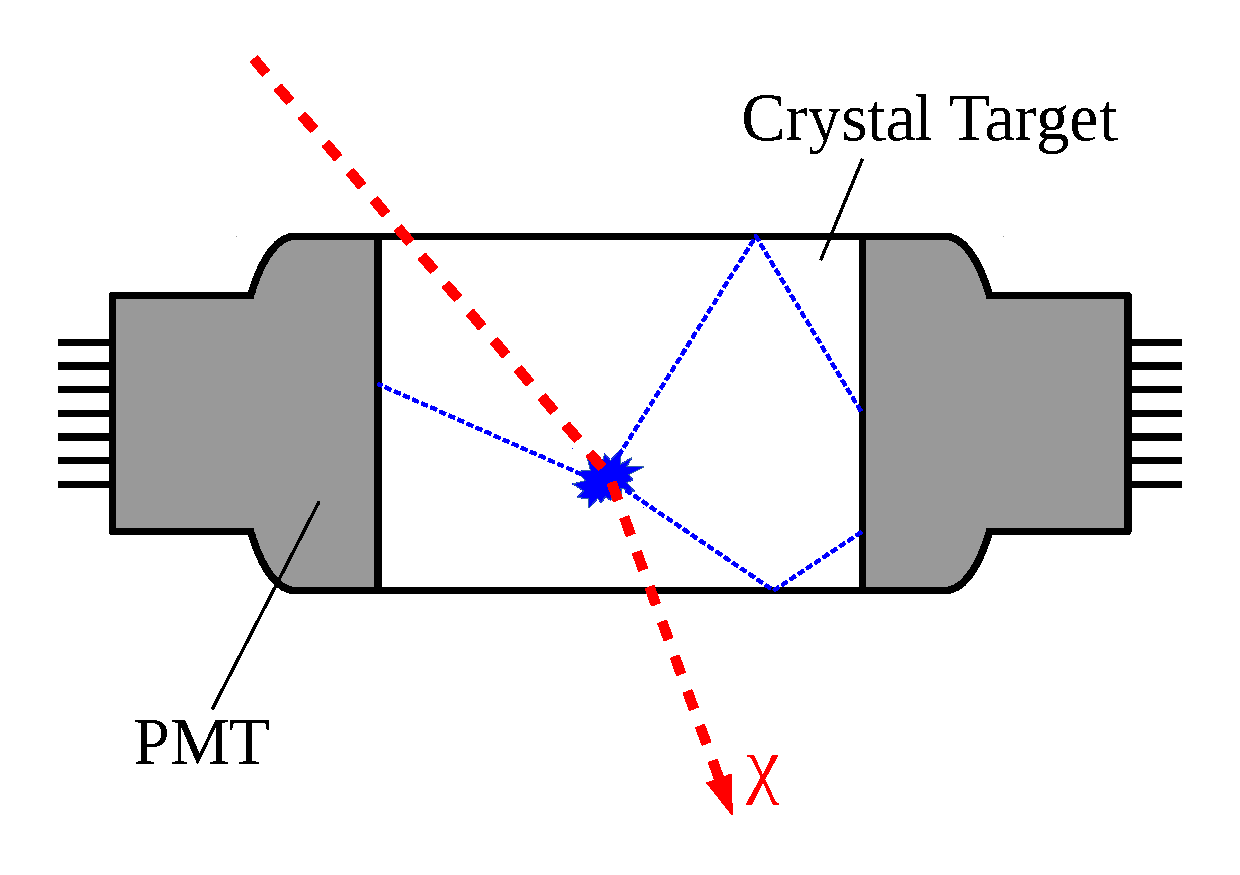
\includegraphics[width=\textwidth]{figures/DMOverview/crystal.pdf}
         \caption{}
         \label{fig:DMOverview/crystal}
     \end{subfigure}
     \hfill
     \begin{subfigure}{0.49\textwidth}
         \centering
         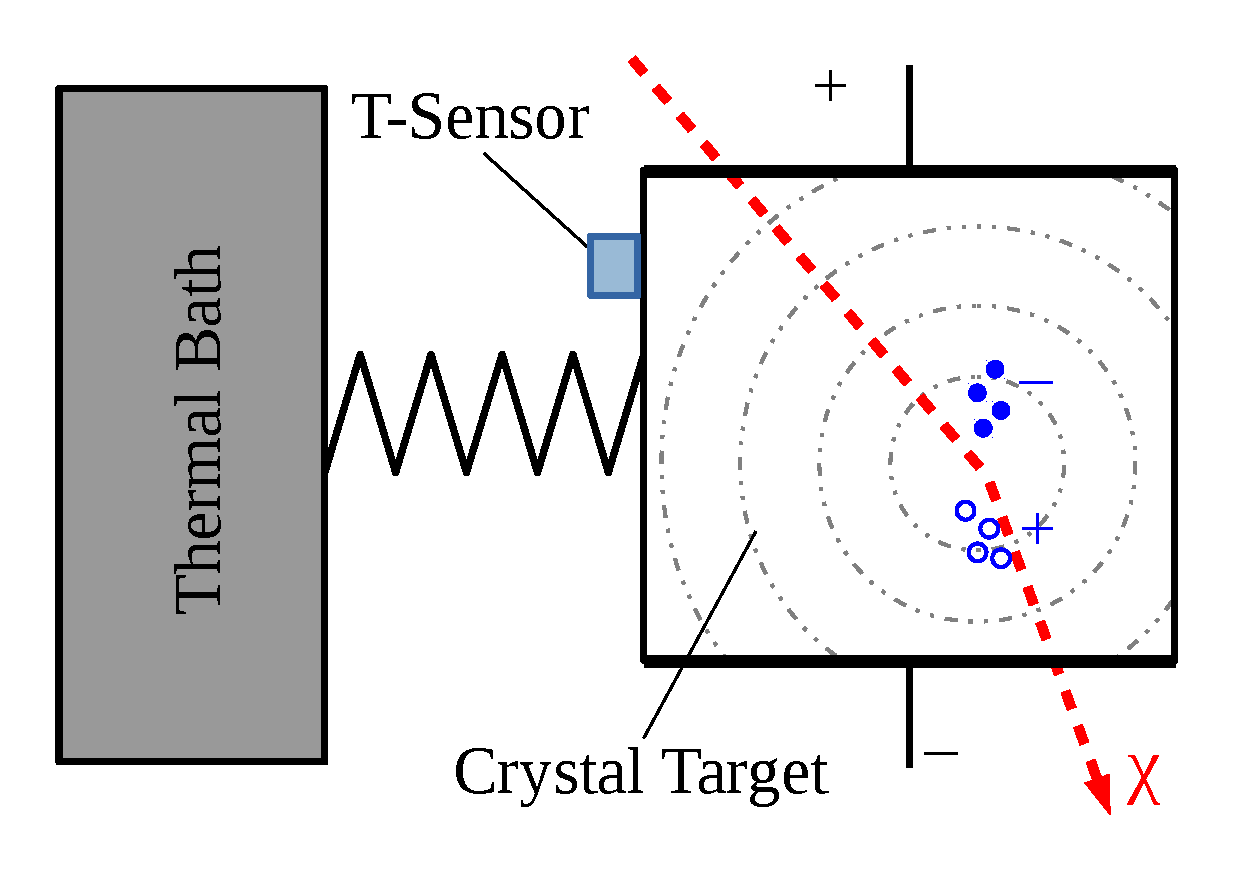
\includegraphics[width=\textwidth]{figures/DMOverview/cryogenic.pdf}
         \caption{}
         \label{fig:DMOverview/cryogenic}
     \end{subfigure}
     \hfill
     \begin{subfigure}{0.49\textwidth}
         \centering
         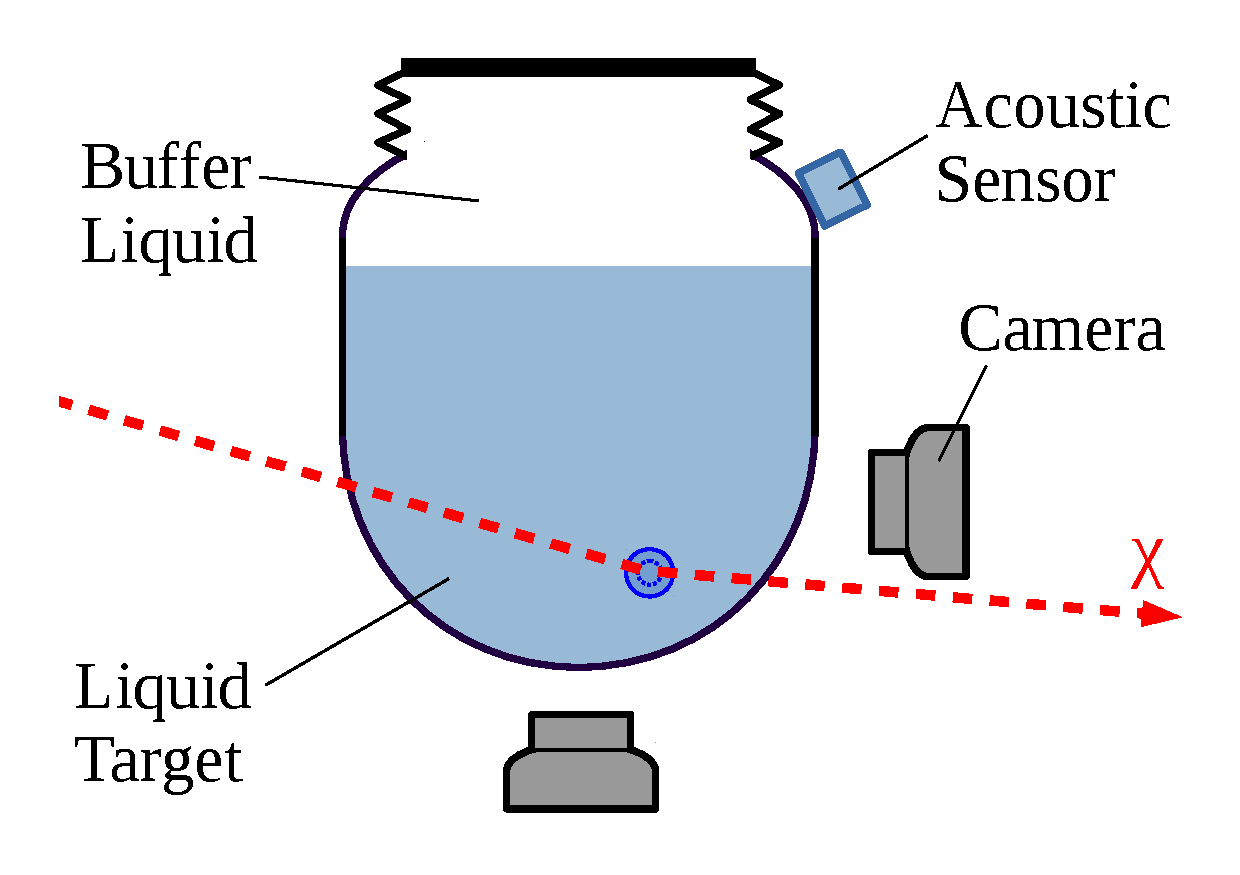
\includegraphics[width=\textwidth]{figures/DMOverview/bubble.pdf}
         \caption{}
         \label{fig:DMOverview/bubble}
     \end{subfigure}
     \hfill
     \begin{subfigure}{0.49\textwidth}
         \centering
         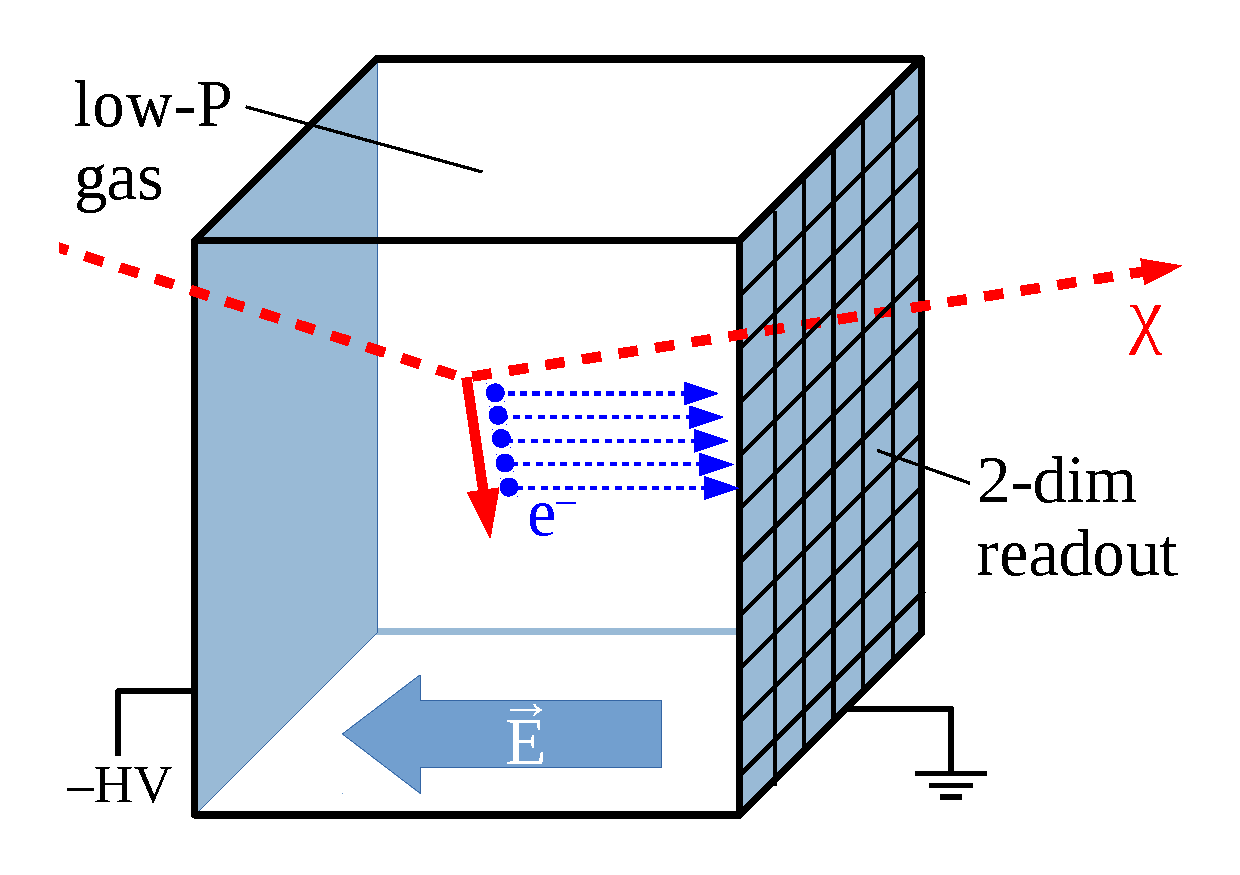
\includegraphics[width=\textwidth]{figures/DMOverview/directional.pdf}
         \caption{}
         \label{fig:DMOverview/directional}
     \end{subfigure}
     \hfill
     \begin{subfigure}{0.49\textwidth}
         \centering
         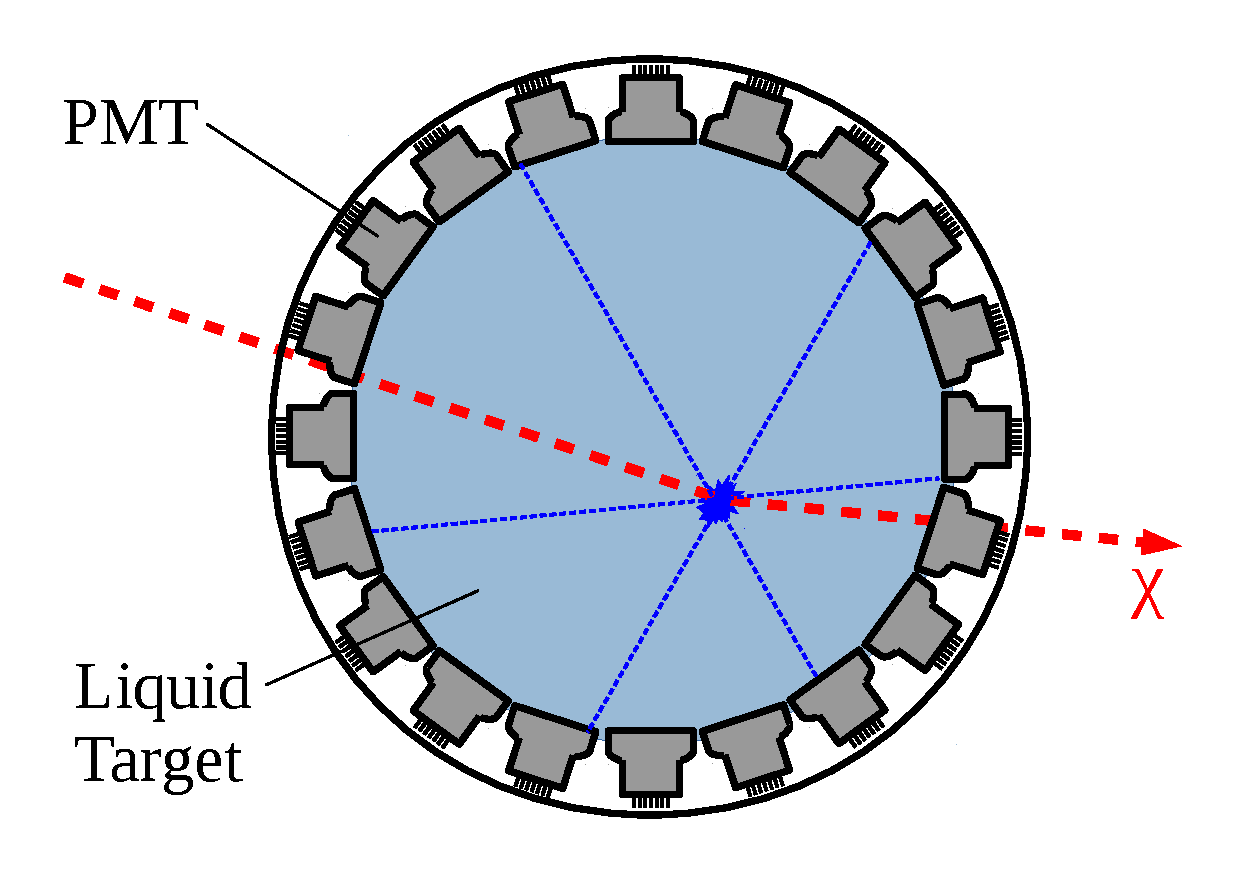
\includegraphics[width=\textwidth]{figures/DMOverview/singlephase.pdf}
         \caption{}
         \label{fig:DMOverview/singlephase}
     \end{subfigure}
     \hfill
     \begin{subfigure}{0.49\textwidth}
         \centering
         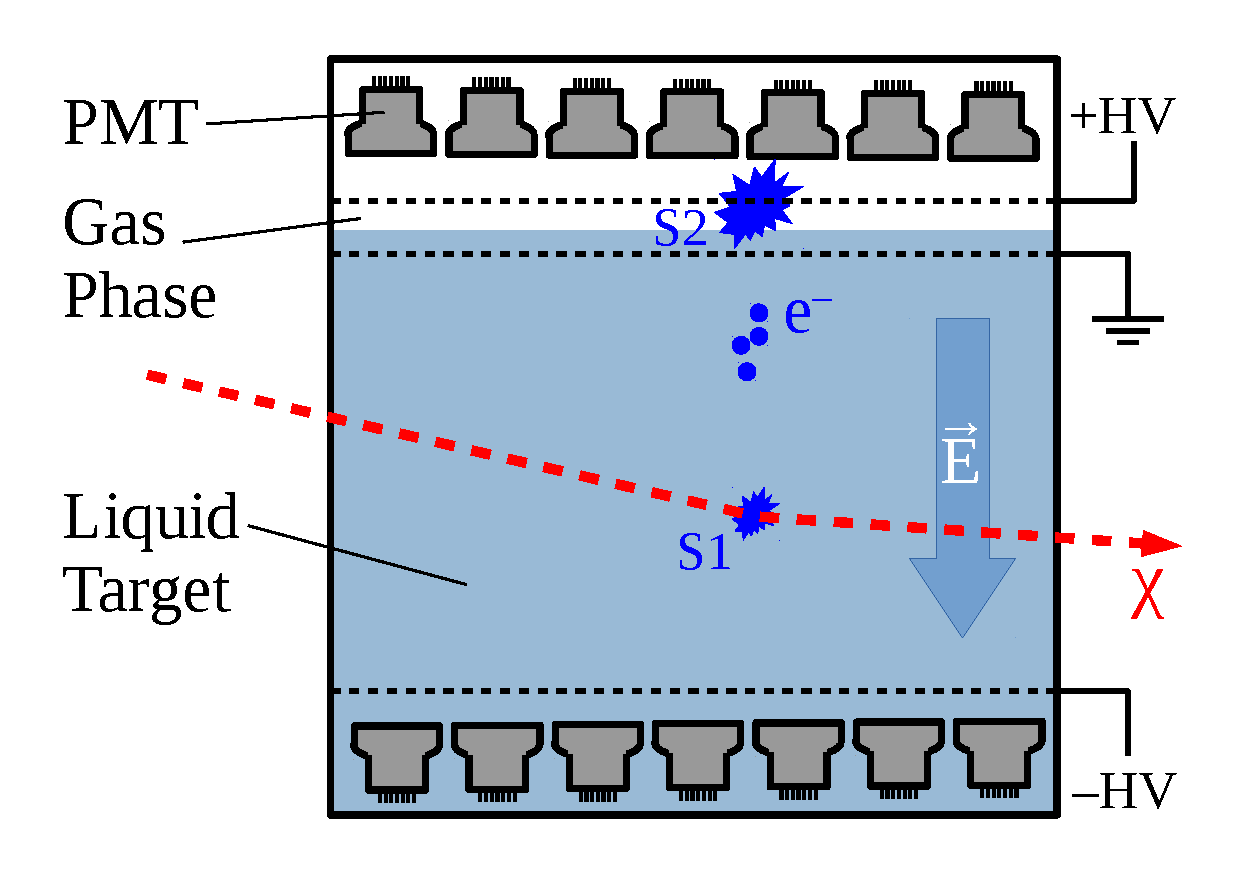
\includegraphics[width=\textwidth]{figures/DMOverview/dualphase.pdf}
         \caption{}
         \label{fig:DMOverview/dualphase}
     \end{subfigure}
     \caption[Schematics of signal readout in different direct detection experiments.]{Schematics of signal readout in different direct detection experiments upon nuclear recoil with dark matter particle $\chi$ (red dashed arrow). Areas of blue indicate a liquid target, white indicates the remaining crystal and gas targets and grey area represents some energy detection device. Each of the six detector types are described in \autoref{sec:DMOverview/DirectDetection}. Figures reprinted from Ref.~\cite{Schumann:2019eaa}.}
     \label{fig:DMOverview/DDSetups}
\end{figure}

\subsubsection{Current status for dark matter searches}\label{sec:DMOverview/DMCurrentStatus}
At the time of writing, no experiment has detected a dark matter particle. However, various experiments have placed increasingly stringent upper limits on the WIMP-nucleon interaction cross-section as a function of WIMP mass, based on data collected over a defined number of ``live days''. The most recent spin-independent WIMP-nucleon cross section limits as a function of WIMP mass are shown in \autoref{fig:DMOverview/WIMPCrossSec.pdf}.
\begin{figure}[ht!]
    \centering
    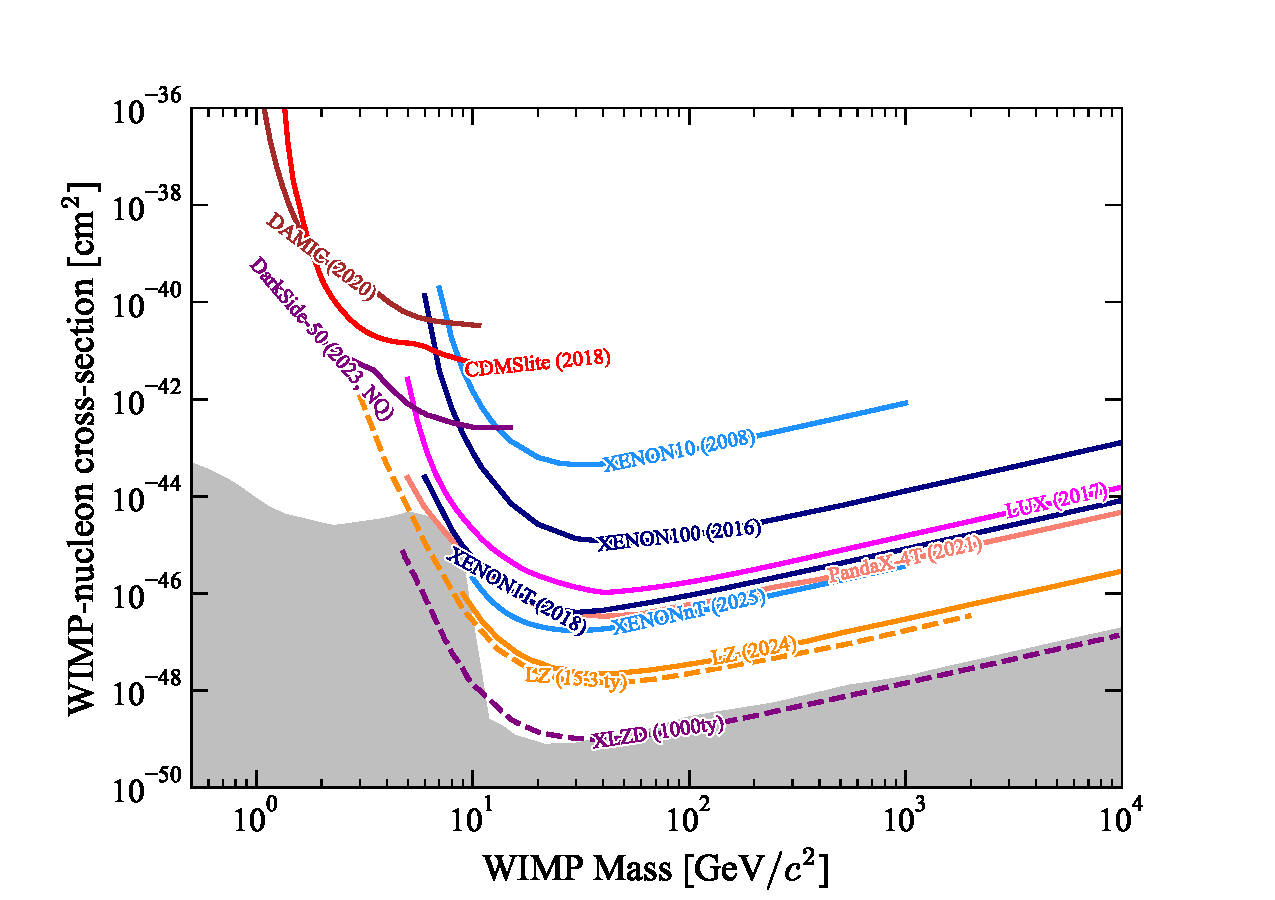
\includegraphics[width=\linewidth]{figures/DMOverview/allwimp_limits.pdf}
    \caption[Most recent spin-independent WIMP-nucleon cross section limits as a function of WIMP mass.]{Most recent spin-independent WIMP-nucleon cross section limits as a function of WIMP mass for liquid xenon direct detection experiments alongside projected limits for current and future experiments. Figure produced using Ref.\cite{DDLimitRepo} includes limits from XENON10 \cite{XENON:2007uwm}, XENON100 \cite{XENON100:2016sjq}, LUX \cite{LUX:2016ggv}, PandaX-4T \cite{PandaX-4T:2021bab}, XENON1T \cite{XENON:2018voc}, XENONnT \cite{XENON:2025vwd}, LUX-ZEPLIN (LZ) experiment \cite{LZCollaboration:2024lux}. Projected limits shown have been produced by LZ \cite{LZ:2018qzl}, DARWIN \cite{DARWIN:2016hyl} and XLZD \cite{XLZD:2024nsu}. The area coloured in grey represents the neutrino floor \cite{Billard:2013qya}.}
    \label{fig:DMOverview/WIMPCrossSec.pdf}
\end{figure}